%%%%%%%%%%%%%%%%%%%%%%%%%%%%%%%%%%%%
% This is the template for submission to ISCA 2016
% The cls file is a modified from  'sig-alternate.cls'
%%%%%%%%%%%%%%%%%%%%%%%%%%%%%%%%%%%%

\documentclass{sig-alternate} 
\usepackage{mathptmx} % This is Times font

\newcommand{\ignore}[1]{}
\usepackage{fancyhdr}
\usepackage[normalem]{ulem}
\usepackage[hyphens]{url}
\usepackage{hyperref}

\usepackage{graphicx}
\usepackage{multirow}
\usepackage{breakurl}
\usepackage{tabularx}
\usepackage[nocompress]{cite}
\usepackage{subfig}
\usepackage{hyphenat}
\usepackage{xcolor}
\usepackage{dcolumn}
\newcolumntype{d}{D{.}{.}{2.1}}
\usepackage{flushend}
 \usepackage{pifont}
\newcommand*\mycirc[1]{{\large \ding{\numexpr201+#1\relax}}}

% required to break long URLS sanely
\PassOptionsToPackage{hyphens}{url} \usepackage{hyperref}
\expandafter\def\expandafter\UrlBreaks\expandafter{\UrlBreaks% save the current one 
\do\a\do\b\do\c\do\d\do\e\do\f\do\g\do\h\do\i\do\j% 
\do\k\do\l\do\m\do\n\do\o\do\p\do\q\do\r\do\s\do\t% 
\do\u\do\v\do\w\do\x\do\y\do\z\do\A\do\B\do\C\do\D% 
\do\E\do\F\do\G\do\H\do\I\do\J\do\K\do\L\do\M\do\N% 
\do\O\do\P\do\Q\do\R\do\S\do\T\do\U\do\V\do\W\do\X% 
\do\Y\do\Z\do\*\do\-\do\~\do\'\do\"\do\-}%

%%%%%%%%%%%---SETME-----%%%%%%%%%%%%%
\newcommand{\hpcasubmissionnumber}{18}
%%%%%%%%%%%%%%%%%%%%%%%%%%%%%%%%%%%%

\fancypagestyle{firstpage}{
  \fancyhf{}
\setlength{\headheight}{50pt}
\renewcommand{\headrulewidth}{0pt}
  \fancyhead[C]{\normalsize{ISCA 2016 Submission
      \textbf{\#\hpcasubmissionnumber} \\ Confidential Draft: DO NOT DISTRIBUTE}} 
  \pagenumbering{arabic}
}  

%%%%%%%%%%%---SETME-----%%%%%%%%%%%%%
\title{Thermostat} 
%\title{Managing Huge Pages In Two-Tiered Main Memory} 
\author{}
%\author{Neha Agarwal, Thomas F. Wenisch\\University of Michigan}
%%%%%%%%%%%%%%%%%%%%%%%%%%%%%%%%%%%%

\begin{document}
\maketitle
\thispagestyle{firstpage}
\pagestyle{plain}

\begin{abstract}
The advent of denser/cheaper memory technologies has renewed interest in
two-tiered main memory schemes, where cold data are shifted to slow memory to
enable greater capacity or reduce cost.  Past research on two-tiered main memory
has assumed a 4KB page size.  However, our recent work demonstrates that 2MB
(transparent) huge pages are performance critical in Cloud applications.  We
propose to develop a transparent huge-page-aware two-tiered memory solution,
targeting virtualized cloud applications, which integrates support for dynamic
page migration and transparent huge pages, achieving both the capacity/cost
advantages of two-tiered memory and performance advantages of huge pages. Hot
regions within otherwise cold huge pages present a central challenge to our
objective. We propose translation facades, a 4KB translation that remaps a
portion of a 2MB mapping with an alternate physical address or permissions, to
facilitate remapping hot portions of cold huge pages.
\end{abstract}

%\vspace{-0.05in}
\section{Introduction}
%\vspace{-0.05in}
GPUs are now ubiquitous in systems ranging from mobile phones to datacenters like 
Amazon's elastic compute cloud (EC2) and HPC installations like Oak Ridge 
National Laboratory's Titan supercomputer.
%In all of these systems, GPUs are increasingly being used for processing beyond
%traditional computer graphics, including image processing, computer vision,
%machine learning, physical dynamics in games, and modeling high energy particle
%interactions. Regardless of the class of system being considered, GPU/CPU
%architectures are evolving towards general-purpose cache coherent non-uniform
%memory access (CC-NUMA) designs with both CPUs  and GPUs being able to access a
%unified globally-addressable memory~\cite{HSA}.  While some of these systems
%may share a single homogeneous pool of memory, an increasing number of systems
%use heterogeneous memory technologies.  Specifically, cost and/or energy
%concerns are driving memory system architects to provide a pool of
%high-bandwidth memory as well as a higher-capacity pool of lower-cost and/or
%lower-power memory.
Figure~\ref{fig:arch} shows several processor and memory topology options that
are likely to be common over the next several years. While traditional systems
are likely to continue using commodity DDR3 and soon DDR4, many future GPUs and
mobile systems are moving to also include higher bandwidth, but capacity
limited, on-package memories such as High Bandwidth Memory (HBM) or Wide-IO2
(WIO2)\@. Regardless the type of machine, both memories will be globally
accessible to maximize aggregate capacity and performance, making all systems
non-uniform memory access (NUMA) due to variations in latency, bandwidth, and
connection topology. Depending on the memories paired the bandwidth ratio
between the bandwidth-optimized (BO) and capacity or cost optimized (CO) memory
pools may be as low as 2$\times$ or as high as 8$\times$.

\begin{figure}[t]
    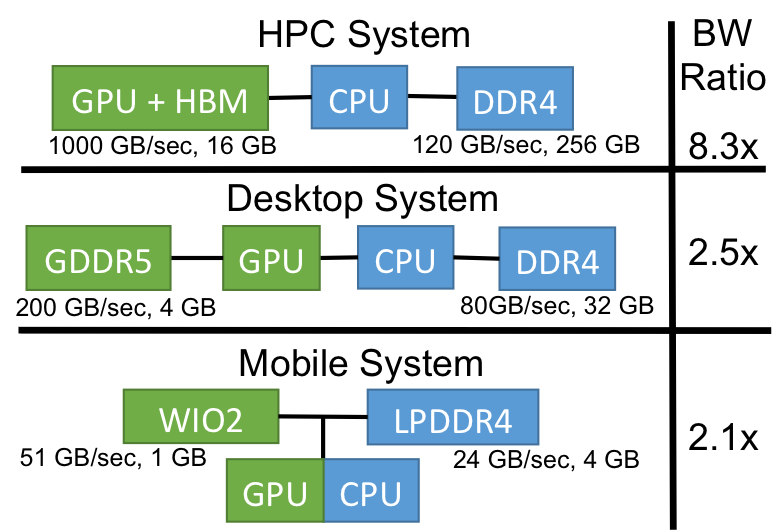
\includegraphics[width=\columnwidth]{asplos2015/figures/arch}
    \caption{BW-Ratio of high-bandwidth vs high-capacity memories for likely future HPC, desktop, and mobile systems}
    \label{fig:arch}
\end{figure}

%To date, GPU-attached bandwidth optimized (BO) memory has been allocated and
%managed primarily as the result of explicit, programmer-directed function calls.
%As heterogeneous GPU/CPU systems move to a transparent unified memory system,
%the OS and runtime systems will become increasingly responsible for memory
%management functions such as page placement, just as they are in CPU-only NUMA
%systems today. In CC-NUMA systems, the notion of local versus remote memory
%latency is exposed to the operating system via the Advanced Configuration and
%Power Interface (ACPI). The latency differences between local and remote memory
%account for the additional latency incurred due to accessing remote memory
%across the system interconnect.  In these systems, latency information, alone,
%is adequate, as CPUs are generally more performance sensitive to memory system
%latency, rather than other memory characteristics.

Massively parallel GPUs and their highly-threaded programming models can
tolerate long memory latencies but, these throughput oriented processors demand
high bandwidth. However, due to lack of exposure of difference in bandwidth
capabilities differential of main memory technologies OS or the programmer, they
cannot make the best memory management decisions to exploit the memory bandwidth
of heterogeneous CPU-GPU system. In this thesis we explore the effect on GPU
performance of exposing memory system bandwidth information to the operating
system/runtime and user applications to improve the quality of dynamic page
placement decisions.

We explore two OS page placement policies:\\
1) Application agnostic Bandwidth-Aware (BW-AWARE) page placement policy that
can outperform Linux's current bandwidth-optimized INTERLEAVE placement by 35\%
and the default latency optimized LOCAL allocation policy by as much as 18\%,
when the application footprint fits within bandwidth-optimized memory capacity.  
\\
2) For \emph{memory capacity constrained} systems (i.e. bandwidth-optimized memory
capacity is insufficient for the workload footprint), we demonstrate that using
simple application annotations to inform the OS/runtime of hot versus
cold data structures can outperform the current Linux
INTERLEAVE and LOCAL page placement policies.  Our annotation
based policy combined with bandwidth information can outperform these
page placement policies by 19\% and 12\% respectively, and get within
90\% of oracle page placement performance.

%Contributions of this work include:
%
%\begin{enumerate}
%\item
%We show that existing CPU-oriented page placement policies are not only 
%sub-optimal for placement in GPU-based systems, but simply do not have the 
%appropriate information available to make informed decisions when optimizing for 
%bandwidth-asymmetric memory.  Exposing additional bandwidth information 
%to the OS, as is done for latency today, will be required for optimized decision 
%making.
%\item 
%Perhaps counter-intuitively we show that, placing all pages in the 
%bandwidth optimized memory is not the best performing page placement 
%policy for GPU workloads.  We propose and {\color{black}simulate} a new bandwidth-aware (BW-AWARE) page 
%placement policy that can outperform Linux's current bandwidth-optimized 
%INTERLEAVE placement by 35\% and the default latency optimized LOCAL allocation 
%policy by as much as 18\%, when the application footprint fits 
%within bandwidth-optimized memory capacity.  
%\item 
%For \emph{memory capacity constrained} systems (i.e. bandwidth-optimized memory
%capacity is insufficient for the workload footprint), we demonstrate that using
%simple application annotations to inform the OS/runtime of hot versus
%cold data structures can outperform the current Linux
%INTERLEAVE and LOCAL page placement policies.  Our annotation
%based policy combined with bandwidth information can outperform these
%page placement policies by 19\% and 12\% respectively, and get within
%90\% of oracle page placement performance.
%\end{enumerate}

\vspace{-.1in}
\section{Motivation and Background}
\label{background}

Heterogeneous CPU--GPU systems have been widely
adopted by the high performance computing community 
and are becoming increasingly common in other computing paradigms.  High performance GPUs have 
developed into stand-alone PCIe-attached accelerators requiring explicit memory 
management by the programmer to control data transfers into the GPU's 
high-bandwidth locally attached memory. As GPUs have evolved, the onus of 
explicit memory management has been addressed by providing a unified shared
memory address space between the GPU and CPU~\cite{UVM,HSA}.  Whereas a single 
unified virtual address space improves programmer productivity, discrete GPU and 
CPU systems still have separate locally attached physical memories, optimized for 
bandwidth and latency respectively. 

Managing the physical location of data, and guaranteeing that reads access 
the most up-to-date copies of 
data in a unified shared memory can be done through the use of page level 
migration and protection. Such mechanisms move data at the OS page granularity between 
physical memories~\cite{UVM}.  With the advent of non-PCIe high bandwidth, low latency
CPU--GPU interconnects, the possibility of performing cache-line, rather than OS-page-granularity, accesses
becomes feasible.  Without OS level page protection
mechanisms to support correctness guarantees, however,  the responsibility of coherence
has typically fallen on hardware cache-coherence implementations.

\ignore{Managing the physical location and coherence guarantee of 
data in a unified shared memory can be done through the use of page level 
migration and protection, which moves data at the OS page granularity between 
physical memories~\cite{UVM}.  With the advent of non-PCIe high bandwidth, low latency,
CPU--GPU interconnects the possibility of performing cache-line based accesses,
rather than OS page granularity, becomes feasible.  Without OS level page protection
mechanisms to support shared memory guarantees however,  the responsibility of coherence
has typically fallen on hardware cache-coherence implementations.}

\begin{table}[t]
\begin{center}
\begin{tabular}{ddd}
 \hline
 \multicolumn{1}{l}{Workload} &   \multicolumn{1}{c}{L1 Hit Rate (\%)}  &  \multicolumn{1}{c}{L2 Hit Rate (\%)}  \\
 \hline
 \hline
 \multicolumn{1}{l}{backprop}  &   62.4  &   70.0\\
 \hline
 \multicolumn{1}{l}{bfs}  &   19.6  &   58.6  \\
 \hline
 \multicolumn{1}{l}{btree}  &   81.8  &   61.8  \\
 \hline
 \multicolumn{1}{l}{cns}  &   47.0  &   55.2  \\
 \hline
 \multicolumn{1}{l}{comd}  &   62.5  &   97.1  \\
 \hline
 \multicolumn{1}{l}{kmeans}  &   5.6  &   29.5  \\
 \hline
 \multicolumn{1}{l}{minife}  &   46.7  &   20.4  \\
 \hline
 \multicolumn{1}{l}{mummer}  &   60.0  &   30.0  \\
 \hline
 \multicolumn{1}{l}{needle}  &   7.0  &   55.7  \\
 \hline
 \multicolumn{1}{l}{pathfinder}  &   42.4  &   23.0  \\
 \hline
 \multicolumn{1}{l}{srad\_v1}  &   46.9  &   25.9  \\
 \hline
 \multicolumn{1}{l}{xsbench}  &   30.7  &   63.0  \\
 \hline
 \hline
 \multicolumn{1}{l}{Arith Mean}  &   44.4  &   51.6  \\
\hline
\end{tabular}
\caption{GPU L1 and L2 cache hit rates (average).}
\label{tab:gpuhitrate}
\end{center}
\vspace{-.25in}
\end{table}

\begin{figure*}[t]
    \centering
    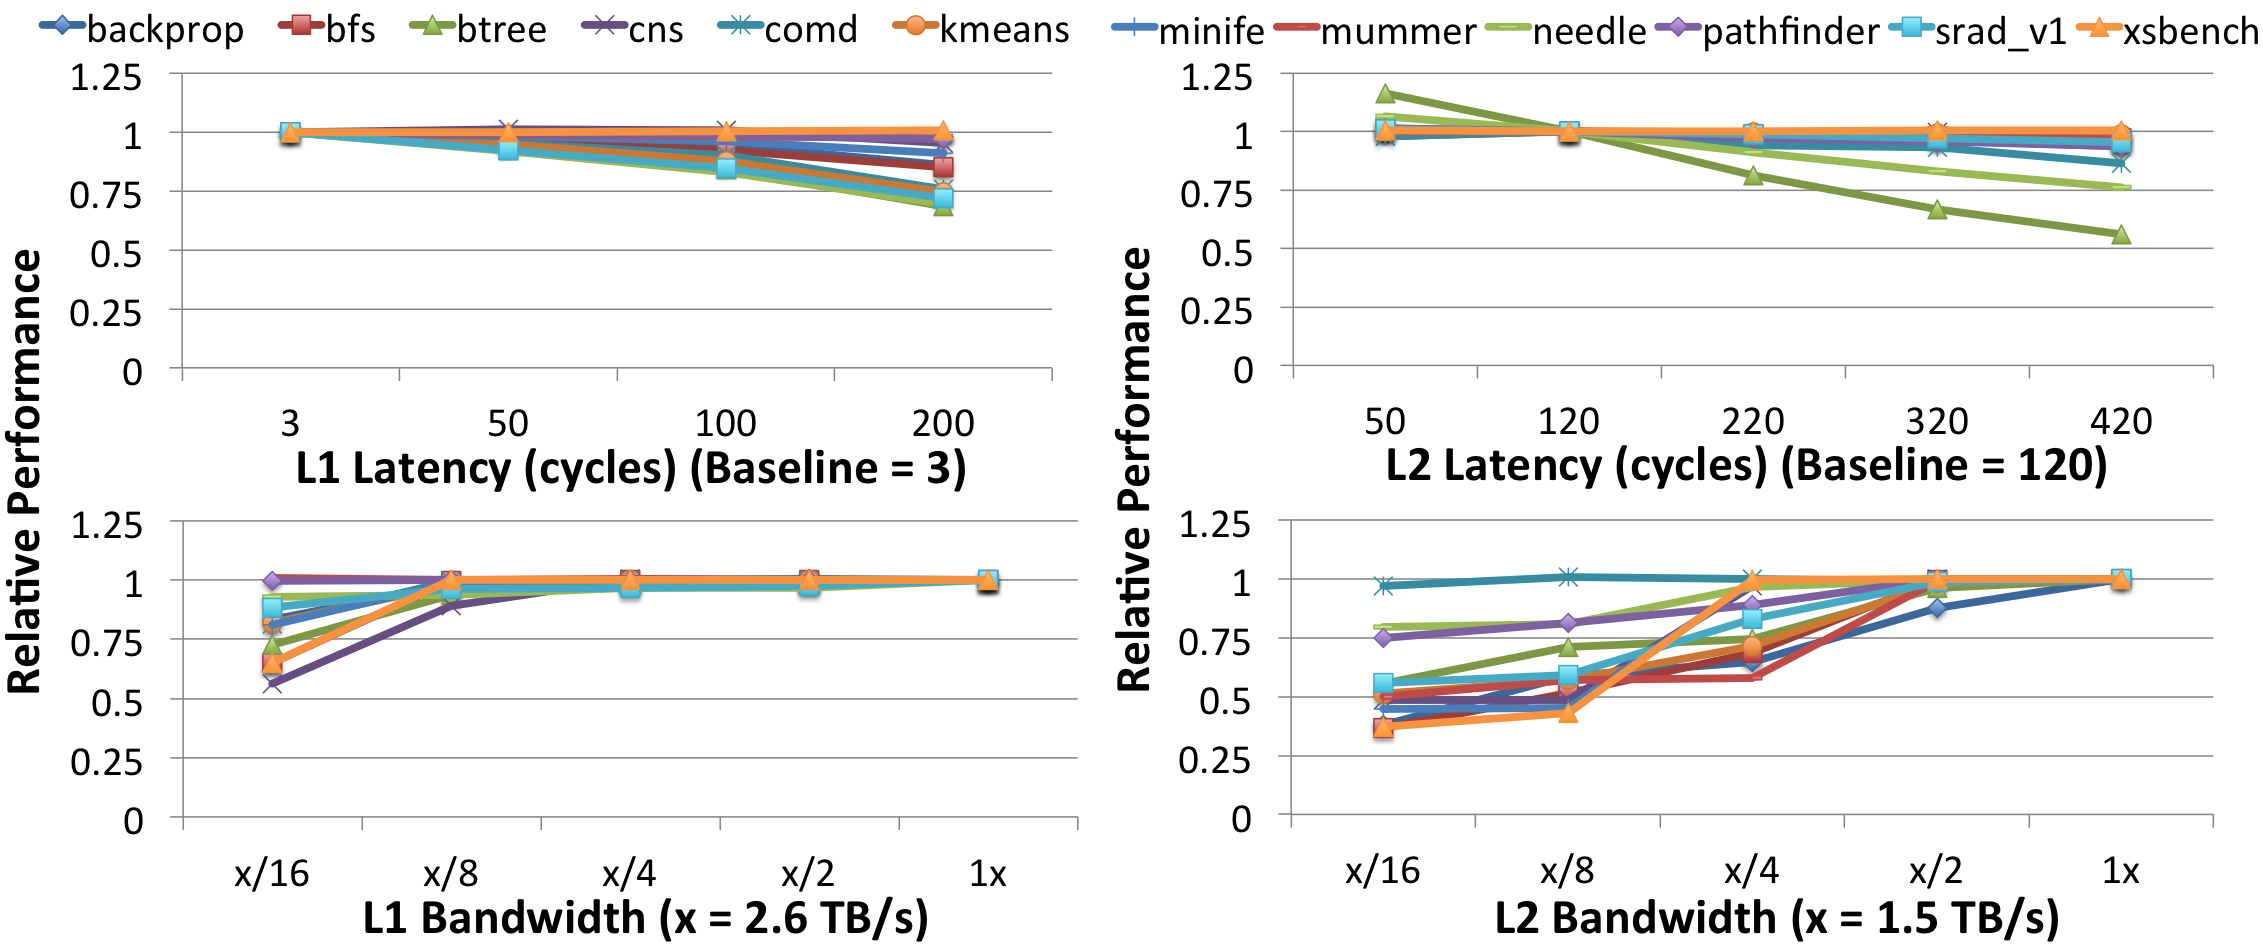
\includegraphics[width=\textwidth]{hpca2016/figures/cache_bw_latency.png}
    \caption{GPU performance sensitivity to L1 and L2 latency and bandwidth
changes.}
    \label{fig:cache_bw_latency}
    \vspace{-.1in}
\end{figure*}

As programming models supporting transparent CPU-GPU sharing become 
more prevalent and sharing becomes more fine-grain and frequent, the 
performance gap between page-level coherence and fine-grained hardware cache-coherent
access will grow~\cite{Agarwal2015,Agarwal2015b,Lim2012}. 
On-chip caches, and thus HW cache coherence, are widely used in CPUs because they 
provide substantial memory bandwidth and latency 
improvements~\cite{Martin2012}.
Building scalable, high-performance cache coherence requires 
a holistic system that strikes a balance between directory storage 
overhead, cache probe bandwidth, and application 
characteristics~\cite{Power2013,Pugsley2010,Cantin2005,johnson2011,Hong2012,Sanchez2012,Kelm2010}.
Although relaxed or scoped consistency models allow coherence operations
to be re-ordered or deferred, hiding latency, they do not obviate the need 
for HW cache coherence. However, supporting a CPU-like HW coherence model
in large GPUs, where many applications do not require coherence, is a tax on GPU designers.  Similarly,
requiring CPUs to relax or change their HW coherence implementations or implement instructions
enabling software management of the cache hierarchy adds significant system complexity.

Prior work has shown that due to their many threaded design, GPUs are 
insensitive to off-package memory latency but very sensitive to off-chip memory 
bandwidth~\cite{Agarwal2015,Agarwal2015b}. Table~\ref{tab:gpuhitrate}
shows the L1 and L2 cache hit rates across a variety of workloads from the Rodinia 
and United States Department of Energy application suites~\cite{Che2009,villa2014}.  These low hit 
rates cause GPUs to also be fairly
insensitive to small changes in L1 and L2 cache latency and bandwidth, as shown in 
Figure~\ref{fig:cache_bw_latency}.  This lack of sensitivity raises the question whether GPUs need 
to uniformly employ on-chip caching of all off-chip memory in order to achieve good performance.  If GPUs do not 
need or can selectively employ on-chip caching, then CPU--GPU systems can be built that
present a unified coherent shared memory address space to the CPU, while not requiring a 
HW cache-coherence implementation within the GPU. 

Avoiding hardware cache coherence benefits GPUs by decoupling them from the coherence protocol 
implemented within the CPU complex, enables simplified GPU designs, and improves
compatibility across future systems. It also reduces the scaling load on the 
existing CPU coherence and directory structures by eliminating the potential addition
of hundreds of additional caches, all of which may be sharing data. Selective caching does not come without
a cost however. Some portions of the global memory space will become un-cacheable
within the GPU\@ and bypassing on-chip caches can place additional load 
on limited off-chip memory resources.  In the following sections, we show that by leveraging
memory request coalescing, small CPU-side caches, improved interconnect efficiency, and
promiscuous read-only caching, selective caching GPUs can perform nearly as well
as HW cache-coherent CPU--GPU\@ systems.

%\vspace{-0.05in}
\section{BW-AWARE Page Placement}
\label{bwawareplacement}
%\vspace{-0.05in}
Using all available memory bandwidth is a key driver to maximizing 
performance for many GPU workloads.
To exploit this observation, we propose a new OS page placement algorithm which
accounts for the bandwidth differential between different bandwidth-optimized and 
capacity-optimized memories
when making page placement decisions.  This section discusses the need,
implementation, and results for a bandwidth-aware (BW-AWARE) page placement
policy for systems where the application footprint fits within BO memory, the
common case for GPU workloads today.  Later in Section~\ref{binaryinstrument},
we discuss an extension to BW-AWARE placement for systems where memory placement
decisions are constrained by the capacity of the
bandwidth-optimized memory.  Both HPC systems trying to maximize in-memory
problem footprint and mobile systems which are capacity limited by cost and
physical part dimensions may soon encounter these capacity constraints with
heterogeneous memories.

\subsection{Bandwidth Maximized Page Placement}
\label{unconstrained}
%\vspace{-0.05in}
The goal of bandwidth-aware page placement is to enable a GPU
to effectively use the total combined bandwidth of {\color{black}\emph{all} the} memory in the
system.  Because GPUs are able to hide high memory latency without stalling
their pipelines, all memories in a system can be used to service GPU requests, 
even when those memories are off-package or require one or more hops
through a system interconnect to access.
To exploit bandwidth-heterogeneous memories,
our BW-AWARE policy places physical memory pages in the ratio of aggregate 
bandwidths of the memories in the system without requiring any knowledge of page
access frequency. Below we derive that this placement policy is optimal for maximizing
bandwidth.

Consider a system with bandwidth-optimized and capacity-optimized
memories with bandwidths $b_B$ and $b_C$ respectively, where unrestricted
capacity of both memories are available. Let $f_B$ represent fraction of data
placed in the BO memory and $1-f_B$ in the CO memory.  Let us assume there are total of
N memory accesses uniformly spread among different pages. Then the total amount
of time spent by the BO memory to serve $N*f_B$ memory accesses is $N*f_B/b_B$ and
that by the CO memory to serve $N(1-f_B)$ memory accesses is $N(1-f_B)/b_C$.  Since
requests to these two memories are serviced in parallel, the total time T to serve the
memory requests is: 
%\[
%T=max(N*f_B/b_B, N(1-f_B)/b_C)
%\]
$$T=max(N*f_B/b_B, N(1-f_B)/b_C)$$
To maximize performance, T must be minimized. Since, $N*f_B/b_B$ and
$N(1-f_B)/b_C$ are linear in $f_b$ and $N*f_B/b_B$ is increasing function while
$N(1-f_B)/b_C$ is decreasing, the minimum of T occurs when both are equal:
%\[T_{opt}=N*f_B/b_B = N(1-f_B)/b_C\]
$$T_{opt}=N*f_B/b_B = N(1-f_B)/b_C$$
Therefore,
%\[f_{Bopt}=b_B/(b_B+b_C)\]
$$f_{Bopt}=b_B/(b_B+b_C)$$

Because we have assumed that all pages are accessed uniformly, the optimal page
placement ratio is the same as the bandwidth service ratio between the bandwidth-optimized
and capacity-optimized memory pools. From this derivation we make two additional
observations.  First, BW-AWARE placement will generalize to an optimal policy
where there are more than two technologies by placing pages in the bandwidth ratio
of all memory pools. Second, a practical implementation
of a BW-AWARE policy must be aware of the bandwidth provided by the various
memory pools available within a system. Hence there is a need for a new System
Bandwidth Information Table (SBIT), much like there is already a ACPI System
Locality 
Information Table (SLIT) which exposes memory latency information to the operating
system today. We will re-visit the assumption of uniform page access later in Section~\ref{annotation}.  

\begin{table}[t]
\begin{center}
\begin{small}
\begin{tabular}{|l|l|}
%\hline
%Simulator & GPGPU-Sim 3.x\\
%\hline
%GPU Arch & NVIDIA GTX-480 Fermi-like\\
%\hline
%GPU Cores& 15 {\color{black}SMs} @ 1.4Ghz\\
%\hline
%L1 Caches & 16kB/SM \\
%\hline
%L2 Caches & Memory Side 128kB/DRAM Channel\\
%\hline
%L2 MSHRs & 128 Entries/L2 Slice\\
%\hline
\hline
\multicolumn{2}{|c|}{Memory system}\\
\hline
GPU-Local GDDR5 & 8-channels, 200GB/sec aggregate\\
\hline
GPU-Remote DDR4& 4-channels, 80GB/sec aggregate\\
\hline
DRAM Timings & \multicolumn{1}{|l|}{RCD=RP=12,RC=40,CL=WR=12}\\
\hline
GPU-CPU &  100 GPU core cycles\\
Interconnect Latency & \\
\hline
\end{tabular}
\caption{Memory system configuration for heterogeneous CPU-GPU system.}
\label{tab:bw-methodology}
\end{small}
\end{center}
\vspace{-0.15in}
\end{table}

\subsection{Experimental Results}
%\vspace{-0.05in}

While it would be ideal to evaluate our page placement policy on a real CC-NUMA
GPU/CPU system with a heterogeneous memory system, such systems are not available today.
Mobile systems containing both ARM CPU cores and NVIDIA GPU cores exist today in products
such as the NVIDIA Shield Portable, but use a single LPDDR3 memory system.
Desktop and HPC systems today have heterogeneous memory attached to CPUs and discrete
GPUs but these processors are not connected through a cache coherent interconnect.  They require explicit user 
management of memory if any data is to be copied from the host CPU memory to the GPU memory or vice versa
over the PCIe interconnect. Pages can not be directly placed into GPU memory on allocation by the operating system.
Without a suitable real system to experiment on, we turned to simulation to evaluate our
page placement improvements.

%\vspace{0.05in}
\subsubsection{Methodology}
To evaluate BW-AWARE page placement, we simulated a heterogeneous memory system
attached to a GPU comprised of both bandwidth-optimized GDDR and
cost/capacity-optimized DDR where the GDDR memory is attached directly to the
GPU\@.  We discuss our baseline simulation environment in
Chapter~\ref{chap:methodology}.
%No contemporary GPU system is available which supports cache-coherent access to
%heterogeneous memories.  Commonly available PCIe-attached GPUs are constrained
%by interconnect bandwidth and lack of cache-coherence; while cache-coherent GPU
%systems, such as AMD's Kaveri, do not ship with heterogeneous memory.  Our
%simulation environment is based on GPGPU-Sim~\cite{gpgpusimIspass09} which has
%been validated against NVIDIA's Fermi class GPUs and is reported to match
%hardware performance with up to 98.3\% accuracy~\cite{gpgpusimManual}.  We
%modified GPGPU-Sim to support a heterogeneous GDDR5-DDR4 memory system with the
%simulation parameters listed in Table~\ref{tab:methodology}.
We model a baseline system with 200GB/s of GPU-attached memory bandwidth and
80GB/s of CPU-attached memory bandwidth, providing a bandwidth ratio of
$2.5\times$\@ as shown in Table~\ref{tab:bw-methodology}.
%We made several changes to the baseline GTX-480 model to bring our
%configuration in-line with the resources available in more modern GPUs,
%including a larger number of MSHRs and higher clock frequency.
With a focus on memory system performance, we evaluate GPU workloads which are
sensitive to memory bandwidth or latency from three benchmark suites:
Rodinia~\cite{Che2009}, Parboil~\cite{Parboil} and recent
HPC~\cite{comd,cns,minife,xsbench} workloads; those which are compute-bound see
little change in performance due to changes made to the memory system.  For the
remainder of the evaluation in this chapter we show results for 19 benchmarks,
17 of which are sensitive to memory bandwidth while also providing {\tt comd}
and {\tt sgemm} results to represent applications which are memory insensitive
and latency sensitive respectively.

%As noted in Section~\ref{heterogeneous_background}, attaching the capacity-optimized memory
%directly to the GPU is functionally equivalent to remote CPU attached memory,
%but with different latency parameters.  To simulate an additional interconnect hop
%to remote CPU-attached memory, we model a fixed, pessimistic, additional 100 cycle latency to access
%the DDR4 memory from the GPU\@. This overhead is derived from the single additional interconnect
%hop latency found in SMP CPU-only designs such as the Intel XEON~\cite{INTELXEON}\@.

%Our heterogeneous memory model contains the same number of MSHRs per memory
%channel as the baseline memory configuration.  The number of MSHRs in the
%baseline configuration is sufficient to effectively hide the additional
%interconnect latency to the DDR memory in Figure~\ref{fig:latency}. Should MSHR
%quantity become an issue when supporting two level memories, previous work has
%shown that several techniques can efficiently increase MSHRs with only modest
%cost~\cite{ref:tuck:scalablemisshandling, ref:minikin:prefetch}.

%Paging model talk
Implementing a BW-AWARE placement policy requires adding another mode ({\tt
MPOL\_BWAWARE}) to the {\tt set\_mempolicy()} system call in Linux\@. When a
process uses this mode, the Linux kernel will allocate pages from the two memory
zones in the ratio of their bandwidths.  These bandwidth ratios may be obtained
from future ACPI resources or dynamically determined by the GPU runtime at
execution time.

\begin{figure}[t]
    \centering
    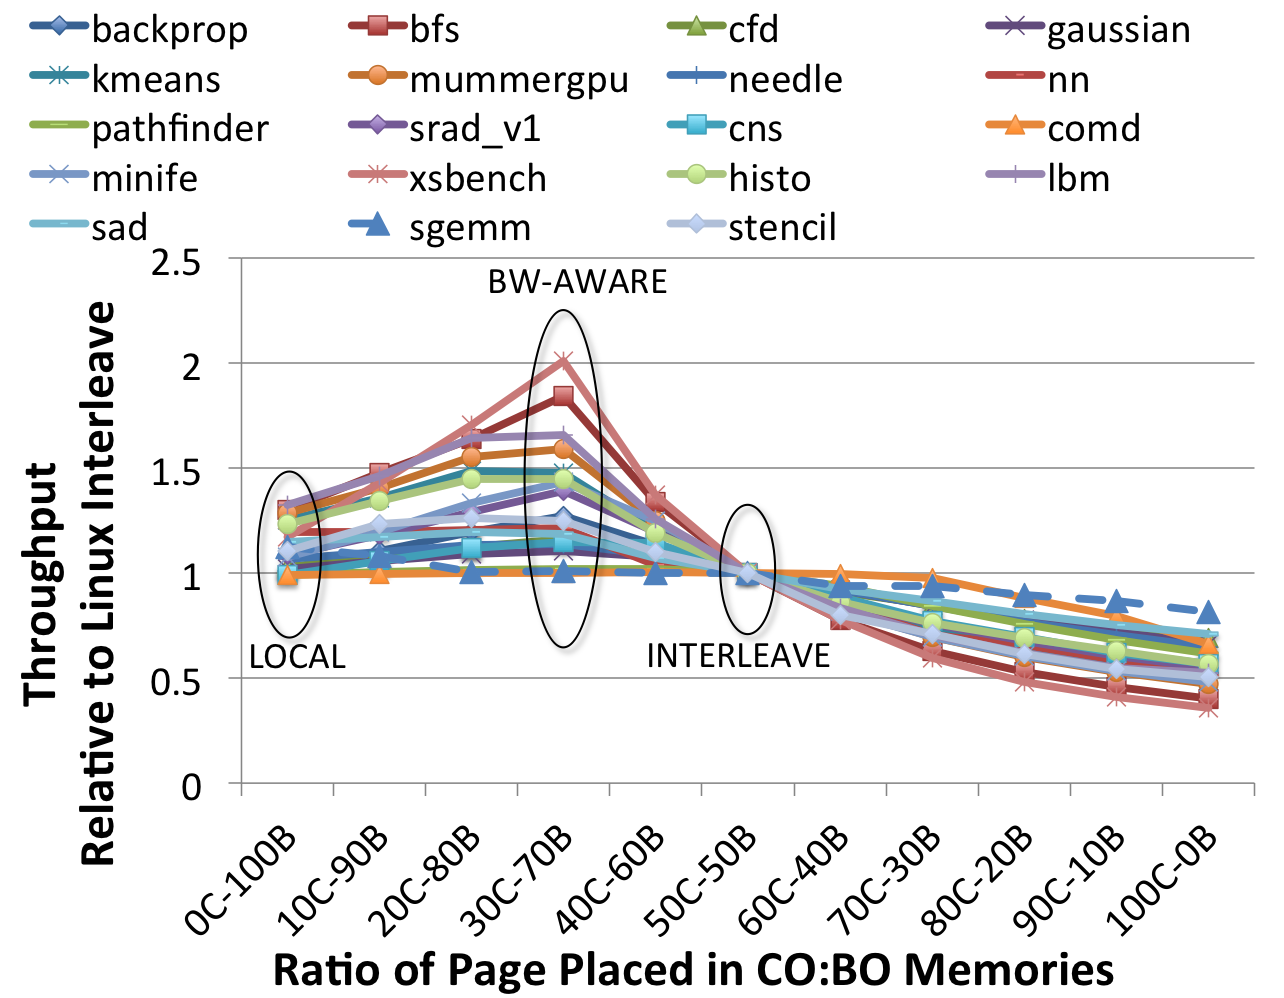
\includegraphics[width=0.9\columnwidth]{asplos2015/figures/bw-aware-2.png} 
    \caption{GPU workload performance with different page placement policies.
$xC$-$yB$ policy represents $x:y$ data transfer ratio from CO and BO memory respectively.}
    \label{fig:baseline}
\end{figure}

%\vspace{0.05in}
\subsubsection{BW-AWARE Performance}
We define our BW-AWARE page placement policy $xC$-$yB$, where $x$ and $y$ denote the
percentage of pages placed in a given memory technology, $C$ stands for capacity-optimized
memory and $B$ stands for bandwidth-optimized memory. By definition $x+y=100$. For our baseline
system with 200GB/sec bandwidth-optimized memory and 80GB/sec of capacity-optimized memory the
aggregate system bandwidth is 280GB/sec.  In this
notation, our BW-AWARE policy will then be $x=80/280=28\%$ and $y=200/280=72\%$, represented as
$28C$-$72B$. However, for simplicity we will round this to $30C$-$70B$ for use as the 
placement policy.  For processes running on the GPU, the LOCAL policy
would be represented as $0C$-$100B$; $50C$-$50B$ corresponds to the bandwidth spreading Linux
INTERLEAVE policy.

To achieve the target $30C$-$70B$ bandwidth ratio, we implemented BW-AWARE placement as follows.
On any new physical page allocation, a random number in the range $[0,99]$
is generated.  If this number is $\geq30$, the page is allocated from the bandwidth-optimized memory; 
otherwise it is allocated in the capacity-optimized memory. A LOCAL allocation policy can avoid the
comparison if it detects either B or C has the value zero.  While this implementation does
not exactly follow the BW-AWARE placement ratio due to the use of random numbers, in practice this 
simple policy converges quickly towards the BW-AWARE ratio.  This approach also requires no history
of previous placements {\color{black} nor makes any assumptions about the frequency of access to pages}, 
minimizing the overhead for making placement decisions which are on the 
software fast-path for memory allocation.

Figure~\ref{fig:baseline} shows the application performance as we vary the ratio of pages placed in 
each type of memory from 100\% BO to 100\% CO\@. 
For all bandwidth-sensitive applications, the maximum performance is
achieved when using the correct BW-AWARE $30C$-$70B$ placement ratio.  We
find that, on average, a BW-AWARE policy performs 18\% better than the Linux
LOCAL policy and 35\% better than the Linux INTERLEAVE policy. However, for latency sensitive
applications, such as {\tt sgemm}, the BW-AWARE policy may perform worse than a LOCAL
placement policy due to an increased number of accesses to higher latency remote
CO memory. The BW-AWARE placement policy suffers a worse case performance degradation of
12\% over the LOCAL placement policy in this scenario.

%This degradation is expected
% since performance degrades by 9\% when the memory latency is 140 cycles
% (Figure~\ref{fig:latency}), which
% is very near to average memory latency (130 cycles = 70\%*100 + 30\%*200).}
%All of the applications we examined appear to be able to tolerate the additional 
%interconnect latency when using a remote capacity-optimized memory.

Because the current Linux INTERLEAVE policy is identical to BW-AWARE for a bandwidth-symmetric
DRAM $50C$-$50B$ memory technology pairing, we believe a BW-AWARE placement policy could simply
replace the current Linux INTERLEAVE policy without having significant negative side
affects on existing CPU or GPU workloads.  Because maximizing bandwidth is more important
than minimizing latency for GPU applications, BW-AWARE placement may be a good candidate
to become the default placement policy for GPU-based applications.
% It is worth noting that there are some GPU applications that are known to be
% sensitive to DRAM latency {\color{red}({\tt sgemm} in our case)}, 
% and using the LOCAL page placement policy may still be preferred.

\begin{figure}[t]
    \centering
    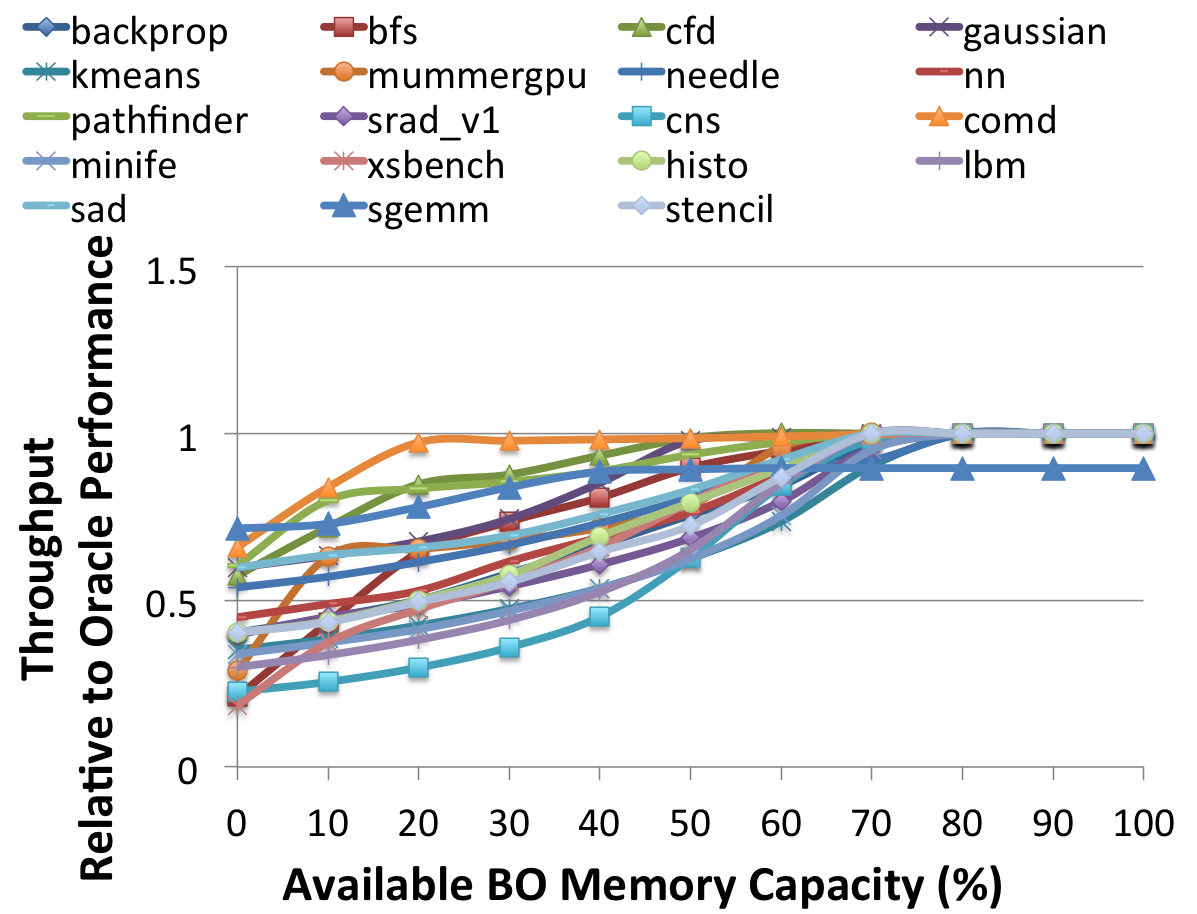
\includegraphics[width=0.9\columnwidth]{asplos2015/figures/bwaware-capacity.png}
    \caption{Performance of BW-AWARE placement as application footprint exceeds
available high-bandwidth
    memory capacity.}
    \label{fig:capacityconstrained}
\end{figure}

%\vspace{0.05in}
\subsubsection{Effective Improvement in Problem Sizing}
Figure~\ref{fig:capacityconstrained} shows the application throughput as we
reduce the capacity of our bandwidth-optimized memory pool as a fraction of the
total application footprint.  BW-AWARE placement is able to achieve near peak
performance even when only 70\% of the application footprint fits within the BO
memory because BW-AWARE placement places only 70\% of pages in BO memory, with
the other 30\% is placed in the less expensive capacity-optimized memory.  Thus,
GPU programmers who today tune their application footprint to fit entirely in
the GPU-attached BO memory could gain an extra 30\% effective memory capacity by
exploiting the CPU-attached CO memory with a BW-AWARE placement policy.
However, as the bandwidth-optimized memory capacity drops to less than 70\% of
application footprint, performance begins to fall off. This effect is due to the
ratio of bandwidth service from the two memory pools no longer matching the
optimal ratio of $30C$-$70B$, with more data being serviced from the capacity
optimized ratio than is ideal. Applications which are insensitive to memory
bandwidth (shown as having little change in Figure~\ref{fig:baseline}), tend to
maintain their performance at reduced capacity points (shown as having little
change in Figure~\ref{fig:capacityconstrained}), because the average bandwidth
reduction does not strongly affect their performance.  Conversely, those
applications with strong BW-performance scaling tend to see larger performance
reduction as the average bandwidth available is reduced, due to capacity
constraints forcing a disproportionate number of memory accesses to the lower
bandwidth CO memory.  The performance at 70\% memory capacity does not exactly
match 100\% of ideal because the actual ratio of bandwidth in our system is
$28C$-$72B$ not $30C$-$70B$.

\begin{figure}[t]
    \centering
    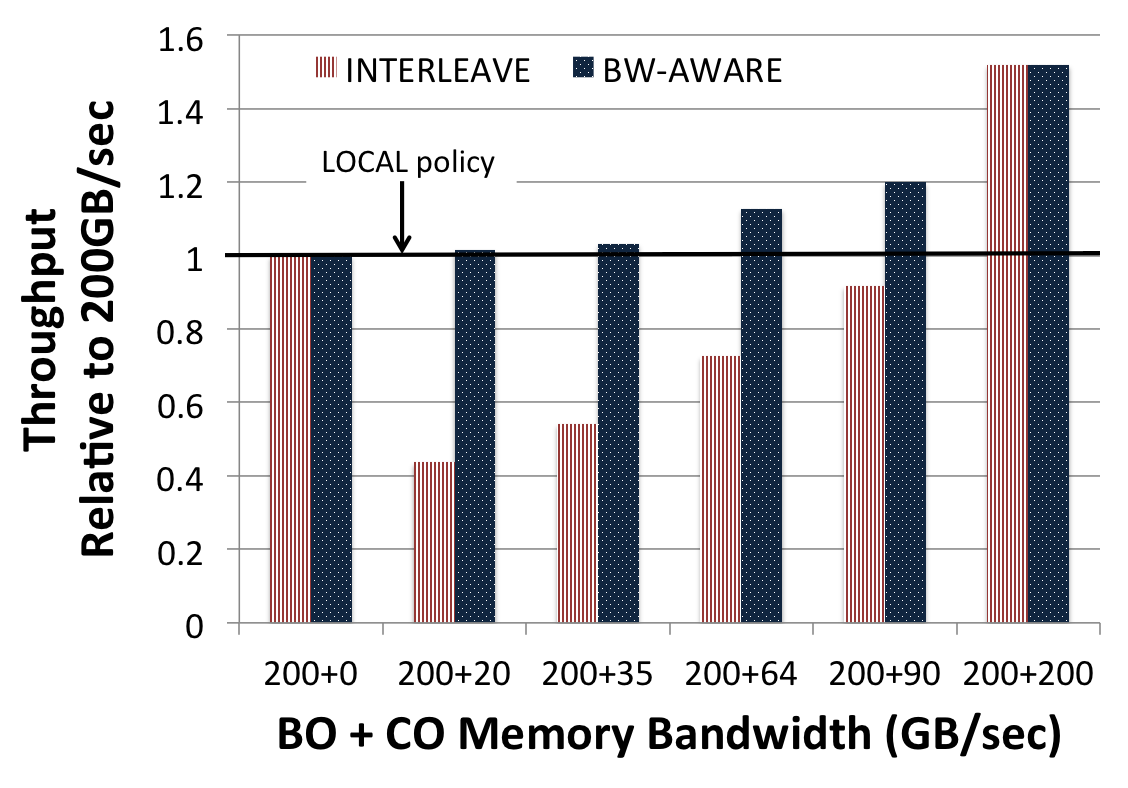
\includegraphics[width=0.9\columnwidth]{asplos2015/figures/sensitivitytobwratio.png}
    \caption{Performance comparison between BW-AWARE, INTERLEAVE, and LOCAL page placement
policies while varying the memory bandwidth ratio.}
    \label{fig:sensitivitytobwratio}
\end{figure}

%\vspace{0.05in}
\subsubsection{Sensitivity to NUMA BW-Ratios} 
Heterogeneous memory systems are likely to come in a variety of configurations.
For example, future mobile products may pair energy efficient and
bandwidth-optimized Wide-IO2 memory with cost-efficient and higher capacity
LPDDR4 memory.  Using the mobile bandwidths shown in
Figure~\ref{fig:arch-asplos2015}, this configuration provides an additional 31\%
in memory bandwidth to the GPU versus using the bandwidth-optimized memory
alone.  Similarly, HPC systems may contain GPUs with as many as 4 on-package
bandwidth-optimized HBM stacks and high speed serial interfaces to bulk capacity
cost/capacity-optimized DDR memory expanders providing just 8\% additional
memory bandwidth.  While we have explored BW-AWARE placement in a desktop-like
use case, BW-AWARE page placement can apply to all of these configurations.  

Figure~\ref{fig:sensitivitytobwratio} shows the average performance of BW-AWARE, INTERLEAVE, and LOCAL
placement policies as we vary the additional bandwidth available from the
capacity-optimized
memory from 0GB/s--200GB/s.
As the bandwidth available from capacity-optimized memory increases, the LOCAL policy
fails to take advantage of it by neglecting to allocate any pages in the capacity-optimized memory.
The Linux INTERLEAVE policy, due to its fixed round-robin allocation, loses performance
in many cases because it oversubscribes the capacity-optimized memory, resulting in less
total bandwidth available to the application.  On the other hand, BW-AWARE placement
is able to exploit the bandwidth from the capacity-optimized memory regardless the 
amount of additional bandwidth available.  Because BW-AWARE placement performs identically to
INTERLEAVE for symmetric memory and outperforms it in all heterogeneous cases, we believe that
BW-AWARE placement is a more robust default policy than INTERLEAVE when considering bandwidth-sensitive 
GPU workloads.

\section{Methodology}
\label{section:methodology}

\subsection{System Configuration}
We study Thermostat on  a 36-core (72 hardware thread) dual-socket
x86 server, Intel Xeon E5-2699 v3, with 512 GB RAM running Linux 4.5.
Each socket has 45MB LLC. There is a 64-entry TLB per core and a shared 1024
entry L2 TLB. Several of our benchmark applications perform frequent I/O and are
highly sensitive to OS page cache performance.
To improve the page cache, we install {\tt hugetmpfs}, a mechanism that
enables use of huge pages for the {\tt tmpfs}~\cite{hughd-hugetmpfs} filesystem. 
We place all files accessed by the benchmarks in {\tt tmpfs}. In the future, we expect
that Linux may natively support huge pages in the page cache for other file
systems.

We run the benchmarks inside virtual machines using the Kernel-based Virtual
Machine (KVM) virtualization platform.  Client threads, which generate traffic to the
servers, are run outside the virtual machine, on the host OS. We run the client threads 
and server VM on the same system and use a bridge network with virtio between host 
and guest so that network performance is not a bottleneck.
We isolate the CPU and
memory of the guest VM and client threads on separate sockets using 
Linux's control group mechanism~\cite{cgroups} to avoid performance interference.  
The benchmark VM is allocated 8 CPU cores, a typical medium-sized cloud 
instance.
We set the Linux frequency governor to ``performance'' to
disable dynamic CPU frequency changes during application runs. 

\subsection{Emulating slow memory: BadgerTrap}
\label{slow-memory}
Dual-technology main memory, in particular Intel/Micron's 3D XPoint memory, 
is not yet available.  
Hence, we use a software technique to emulate slow memory while placing all
data in conventional DRAM.

Each cache miss to slow memory should incur an access latency that is a multiple 
of the DRAM latency (e.g., 400ns slow memory~\cite{ref:Dulloor:datatiering} vs. 
50ns DRAM latency).
There is no easy mechanism to trap to software on all cache misses. Instead,
we introduce extra latency by inducing page faults upon translation misses (TLB misses) 
to cold pages by using BadgerTrap~\cite{ref:badgertrap}. 
%This mechanism is similar to 
%how Thermostat measures page access frequency.

The software fault mechanism is an approximation of an actual slow memory device.
The BadgerTrap fault latency (about 1us in our kernel) is higher than some authors
predict the 3D XPoint memory read latency will be~\cite{ref:Dulloor:datatiering}.  Furthermore, the poisoned PTE
will induce a fault even if the accessed memory location is present in the hardware 
caches. In these two respects, our approach over-estimates the penalty of slow 
memory accesses.  However, once BadgerTrap installs a (temporary) translation, 
further accesses to other cache blocks on the same slow-memory page will not 
induce additional faults, potentially under-estimating impact. Our testing with micro benchmarks
indicates our approach yields an average access latency to slow memory in the 
desired range, in part, because slow-page accesses are sufficiently infrequent that
they nearly always result in both cache and TLB misses anyway, as we discuss in
Section~\ref{section:access-counting}.
%On balance, we expect the differences between
%TLB and cache misses to have little impact because, by design, Thermostat places
%only rarely accessed pages in cold memory.

%We validate that BadgerTrap provides a reasonable approximation of slow memory
%by measuring the TLB and cache miss rates for our benchmark suite using hardware
%performance counters.  The TLB miss rate induced by BadgerTrap is typically higher 
%(but always within a factor of two) than the last-level cache miss rate measured 
%without BadgerTrap, indicating that our performance estimates are conservative.
%\fixme{Neha: Verify this number for all the new benchmarks.}

One important detail of our test setup is that we must install BadgerTrap (for the purpose 
of emulating slow memory latency) within
the guest VM rather than the host OS.  Thermostat communicates with the guest-OS 
BadgerTrap instance to emulate migration to slow memory.  We must install
BadgerTrap within the guest because, otherwise, each BadgerTrap fault would 
result in a {\tt vmexit}.  In addition to drastically higher fault latency, {\tt vmexit} operations
have the side-effect of changing the Virtual Processor ID (VPID) to 0. Since KVM
uses VPIDs to tag TLB entries of its guests, installing a TLB entry with the
correct VPID would entail complexity and incur even higher emulation latency.
% than
%involve a significantly complex operation of re-entering the
%VM, performing a single memory operation and jumping back, which would incur
%even more emulation latency.
Since BadgerTrap on the guest entails a latency of
$\approx$ 1$\mu$s, which is already higher than projected slow-memory latencies~\cite{ref:Dulloor:datatiering},
we did not want to incur additional slowdown by emulating slow memory in the
host OS.


%To ensure that this approach is
%reasonable, we obtained the TLB and cache miss rates for the applications under
%study by {\tt perf}. We observed that in Cassandra and MySQL-TPCC the TLB miss
%rate (resulting into page walks)
%was 2$\times$ higher than the last level cache miss rate, meaning that we will only be
%overestimating the performance impact. In Redis, however, the TLB miss rate is
%2$\times$ lower than the cache miss rate. 

%{\textbf{Why not Badgertrap on the host?}


\subsection{Benchmarks}
\label{benchmarks}
We evaluate Thermostat with applications from Google's Perfkit Benchmarker and
the Cloudsuite benchmarks~\cite{perfkitbenchmarker, cloudsuite}. These
applications are representative server workloads that have large memory
footprints and are commonly run in virtualized cloud environments.  We do not
evaluate Thermostat for general-purpose GPU applications since non-volatile memory
technologies are expected to have much lower bandwidth than high-bandwidth
graphics memories -- even lower than DDR memory technologies -- thus are not a
suitable match to memory bandwidth-sensitive platforms like GPUs.

{\bf TPCC on MySQL:} TPCC is a widely-used database benchmark, which aims to measure
the transaction processing throughput of a relational database~\cite{tpcc}. We 
execute TPCC on top of MySQL, one of the most popular open-source database 
engines, which is often deployed in the cloud.  We use the open-source
TPCC implementation from OLTP-Bench~\cite{oltpbench} (available at
\url{https://github.com/oltpbenchmark/oltpbench}). We use a scale factor of
320, and run the benchmark for 600 seconds after warming up for 600 seconds.
MySQL makes frequent I/O requests and hence benefits markedly from our use
of {\tt hugetmpfs} to enable huge pages for the OS page cache.
%We observe 380
%transactions/sec throughput for our baseline system with all pages in DRAM as
%huge pages.

{\bf NoSQL databases:} Aerospike, Cassandra, and Redis are popular NoSQL
databases~\cite{aerospike, cassandra, redis}.
Cassandra is a wide-column database designed to offer a variable number of fields
(or columns) per key, while Redis and Aerospike are simpler key-value databases 
that have higher peak throughput. Redis is single-threaded whereas Aerospike is
multi-threaded.
Cassandra performs frequent file I/O as it periodically compacts its SSTable
data structure on disk~\cite{ref:sstable}. So, Cassandra also benefits substantially
from {\tt hugetmpfs}. Redis performs no file I/O after loading its dataset into memory.

We tune Aerospike, Cassandra, and Redis based on the settings provided by
Google's Perfkit Benchkmarker for measuring cloud
offerings~\cite{perfkitbenchmarker}.  We use the YCSB traffic generator to drive
the NoSQL databases~\cite{ycsb}. For Aerospike we use 200M operations
and for Cassandra we use 50M operations on 5M keys with 20 fields each with a
Zipfian distribution.
For both of these application, we evaluate two workload mixes: a read-heavy load
with 95:5 read/write ratio and a write-heavy load with 5:95 read/write ratio. For Redis, we
access keys with a hotspot distribution, wherein 0.01\% of the keys account for
90\% of the traffic. We vary value sizes according to the
distribution reported in~\cite{facebook-key-value}. We observe 176K
and 215K operations/sec for read-heavy and write-heavy workloads for Aerospike,
and 21K and 45K operations/sec for read-heavy and write-heavy workloads for
Cassandra. For Redis we observe 188K
operations/sec for our baseline system with all pages in
DRAM as huge pages.

{\bf In-memory analytics:} We evaluate Thermostat on in-memory analytics
benchmarks from Cloudsuite~\cite{cloudsuite}. In-memory analytics runs a
collaborative filtering algorithm on a dataset of user-movie ratings.  It uses
the Apache Spark framework to perform data analytics. We set both executor and driver
memory to be 6GB to execute the benchmark entirely in memory. We run the benchmark to
completion, which takes 317 seconds for our baseline system with all pages in
DRAM as huge pages.

{\bf Web search:} Cloudsuite's web search uses the Apache Solr search engine
framework. We run client threads on host and index nodes within the virtual
machine. We set steady state time to be 300 seconds and keep default values for all
the other parameters on the client machine. As specified by the benchmark,
target response time requires 99\% of the requests to be serviced in 200ms. For
our baseline system with all pages in DRAM as huge pages, we observe 50
operations/sec with $\approx$ 85ms 99th percentile latency.
%{\bf Tomcat:} Tomcat is a popular web server frontend. We use the {\tt wrk}
%(available at \url{https://github.com/wg/wrk}) tool to generate XXX requests to
%the webpage \texttt{XXX.XXX} using XXX parallel clients. Our installation runs
%at the peak throughput at this load. 

\subsection{Runtime overhead of Thermostat Sampling}
We measure the runtime overhead of Thermostat to ensure that application 
throughput is not degraded by Thermostat's page sampling mechanism.
For sampling periods of 10s or higher, we observe negligible CPU activity
from Thermostat and no measurable application slowdown ($<$ 1\%).


\begin{table}[t]
\begin{center}
\begin{tabular}{|l|l|l|}
\hline
& Resident Set Size& File-mapped\\
\hline
Aerospike & 12.3GB & 5MB\\
\hline
Cassandra & 8GB & 4GB\\
\hline
MySQL-TPCC & 6GB & 3.5GB\\
\hline
Redis & 17.2GB & 1MB\\
\hline
%Graph-analytics & 16.6GB & 1MB\\
%\hline
In-memory-analytics & 6.2GB & 1MB\\
\hline
Web-search & 2.28GB & 86MB\\
\hline
\end{tabular}
%\vspace{0.05in}
\caption{Application memory footprints: resident set size and file-mapped pages.}
\label{tab:memory-footprint}
\end{center}
\end{table}

\section{Evaluation}
\label{results}

We next measure Thermostat's automatic hot/cold classification and run-time
placement/migration mechanisms on our suite of cloud applications.

Thermostat takes as input a tolerable slowdown; a single input parameter 
specified by a system administrator.  It then automatically selects cold pages
 to be migrated to slow memory at runtime. We set a tolerable slowdown of
3\% throughout our evaluation, since a higher slowdown may lead to an overall
cost increase due to higher required CPU provisioning (which is more expensive
than memory). Thermostat's slowdown threshold can be 
changed at runtime through the Linux cgroup mechanism. Hence,
application administrators can
dynamically tune the threshold based on service level agreements
for latency-critical applications or for the throughput requirements of
batch jobs.  We show that, for our application suite, Thermostat meets the
target 3\% slowdown while placing a significant fraction of application footprint in slow memory
dynamically at runtime.

%Based on the characterization results shown in Figure~\ref{fig:cassandra-hotspot},
%we set an objective of migrating roughly half of the application memory footprint
%to slow memory with an expected performance degradation of 5\% for Cassandra
%and TPCC.  However, for Redis, the memory access locality pattern is flat, and
%a 5\% degradation target allows only a small fraction of the footprint to be classified
%as cold.  Hence, for Redis, we set a 10\% degradation target.

We evaluate Thermostat with 5\% of huge pages sampled in every scan interval of
30s and at most 50 4KB pages poisoned for a sampled huge page.
We compare the performance of Thermostat with a placement policy that
places all pages in DRAM, which maximizes performance while incurring maximal 
memory cost.  Thermostat's sampling mechanisms incur a negligible performance
impact (well under 1\%)---the slowdowns we report are entirely attributable to 
slow memory accesses. 

We briefly discuss our findings for each application. Table~\ref{tab:memory-footprint} reports each 
application's footprint in terms of resident set size (RSS) and file-mapped
pages. The memory savings quoted for each benchmark is the average cold memory
fraction over the benchmark's runtime.

\begin{figure}[t]
\centering
%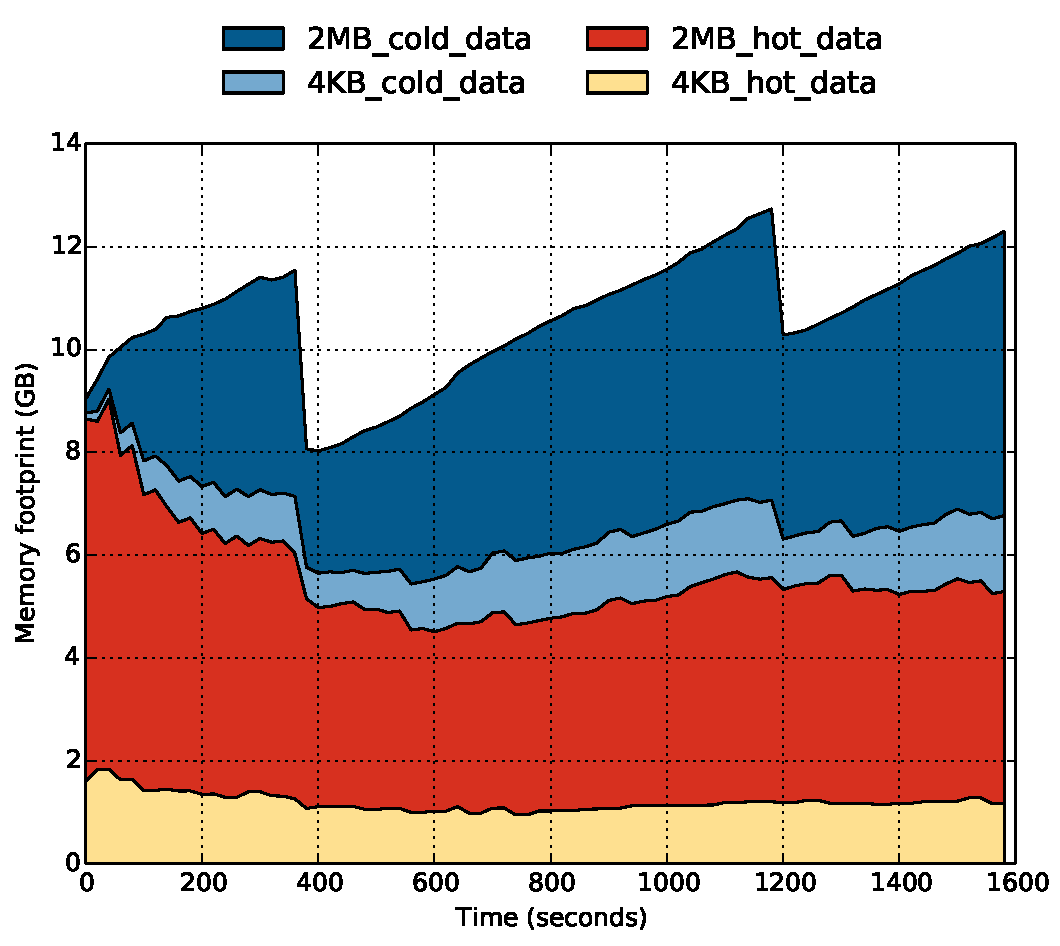
\includegraphics[width=1.0\columnwidth]{figures/cassandra-capacity.pdf}
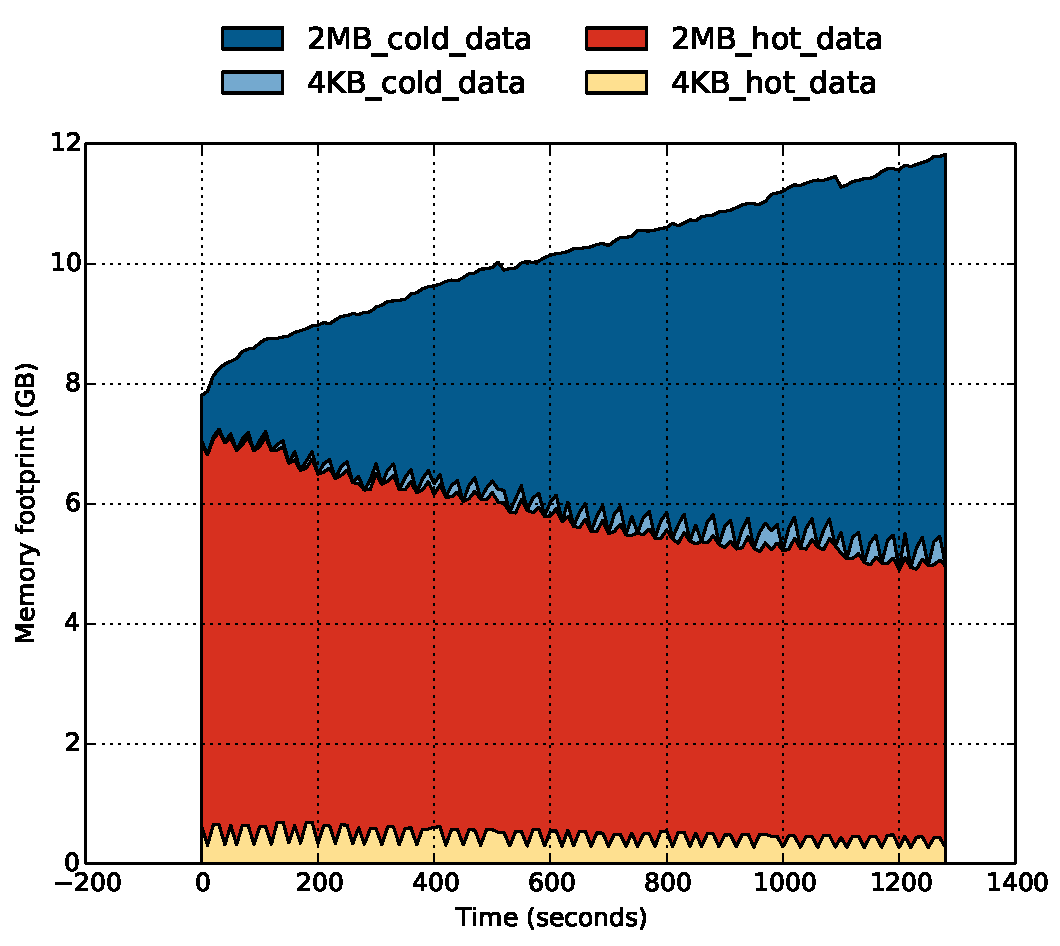
\includegraphics[width=0.8\columnwidth]{asplos2017/figures/cassandra-new-set-policy-kstaled10-sample5-period3-capacity_over_time.pdf}
\caption{Amount of cold data in Cassandra identified at run time with 2\%
throughput degradation for a write-heavy workload (5:95 read/write ratio).}
\label{fig:cassandra-capacity}
\end{figure}

\begin{figure}[t]
\centering
%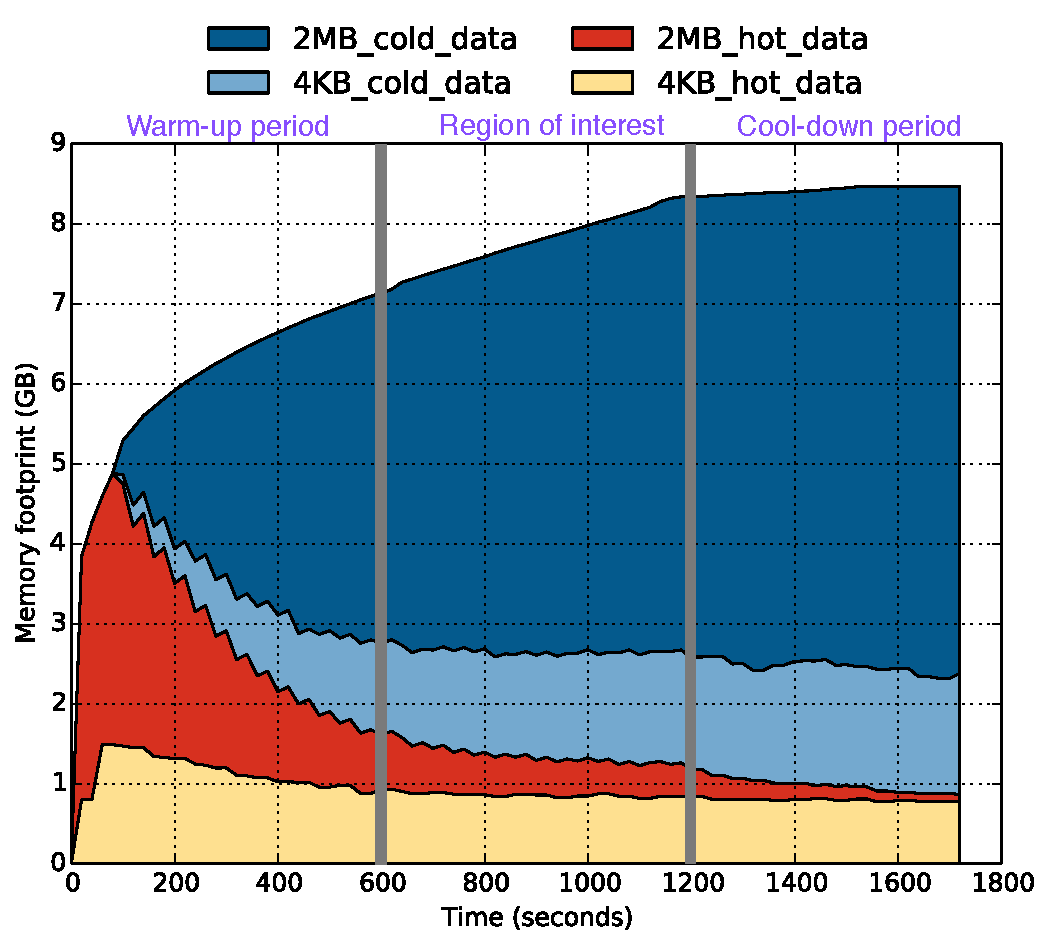
\includegraphics[width=1.0\columnwidth]{figures/tpcc-capacity.pdf}
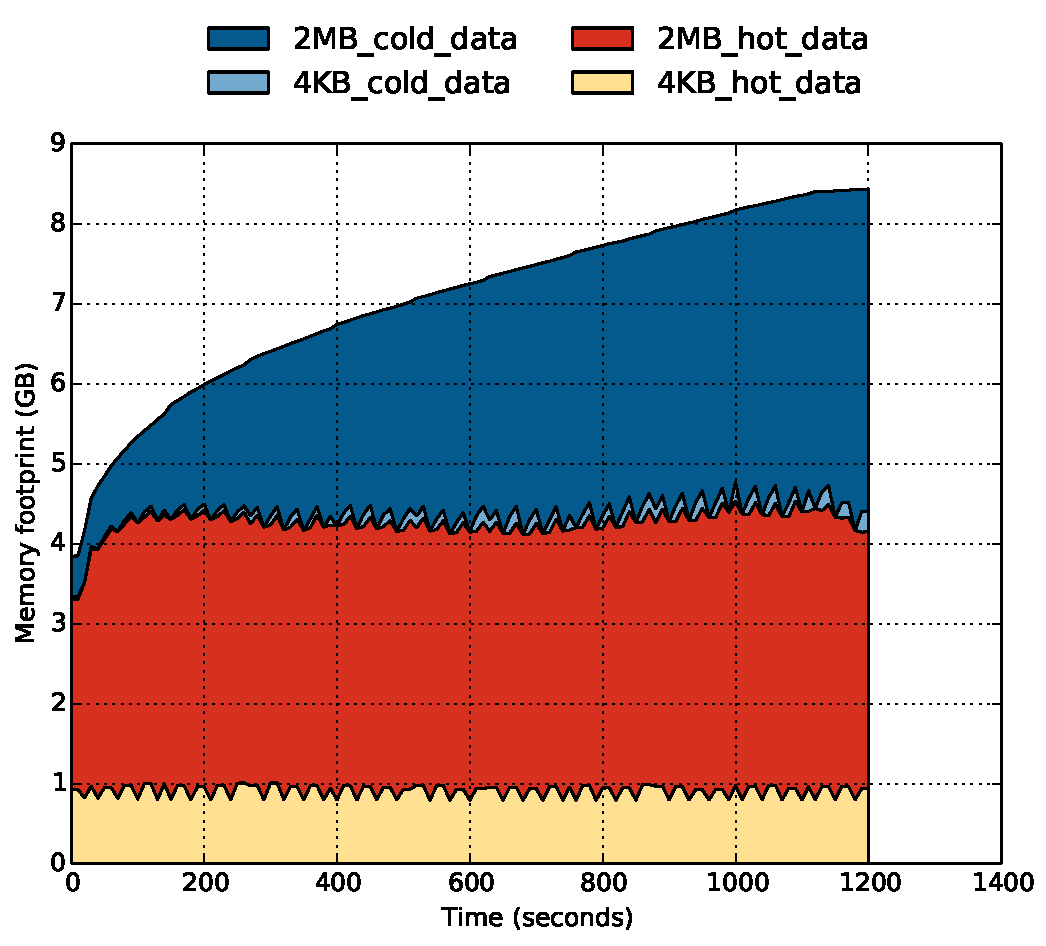
\includegraphics[width=0.8\columnwidth]{asplos2017/figures/tpcc-clipped-new-policy-capacity_over_time.pdf}
\caption{Amount of cold data in MySQL-TPCC identified at run time with 1.3\%
throughput degradation.}
\label{fig:tpcc-capacity}
\end{figure}

\begin{figure}[t]
\centering
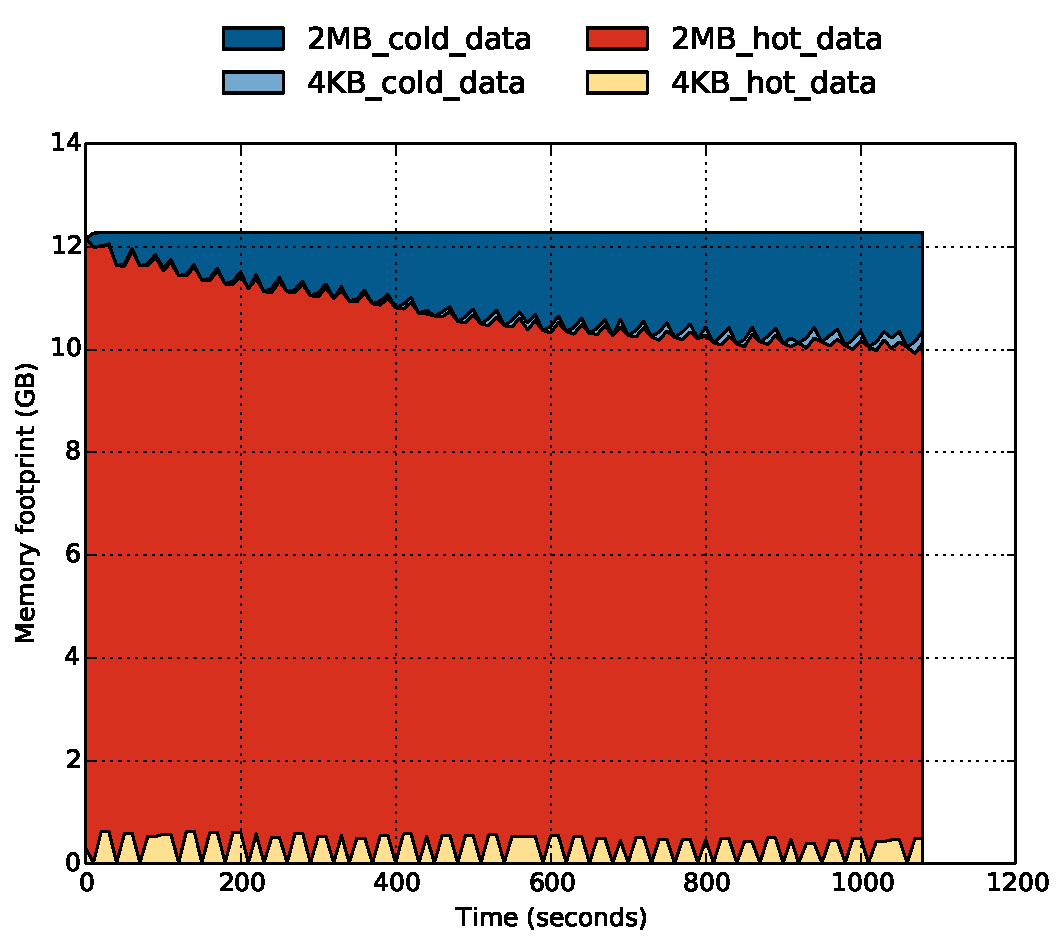
\includegraphics[width=0.8\columnwidth]{asplos2017/figures/aero-new-policy-24perSlow-capacity_over_time.pdf}
\caption{Amount of cold data in Aerospike identified at run time with 1\%
throughput degradation for a read-heavy workload (95:5 read/write ratio).}
\label{fig:aerospike-capacity}
\end{figure}

\begin{figure}[t]
\centering
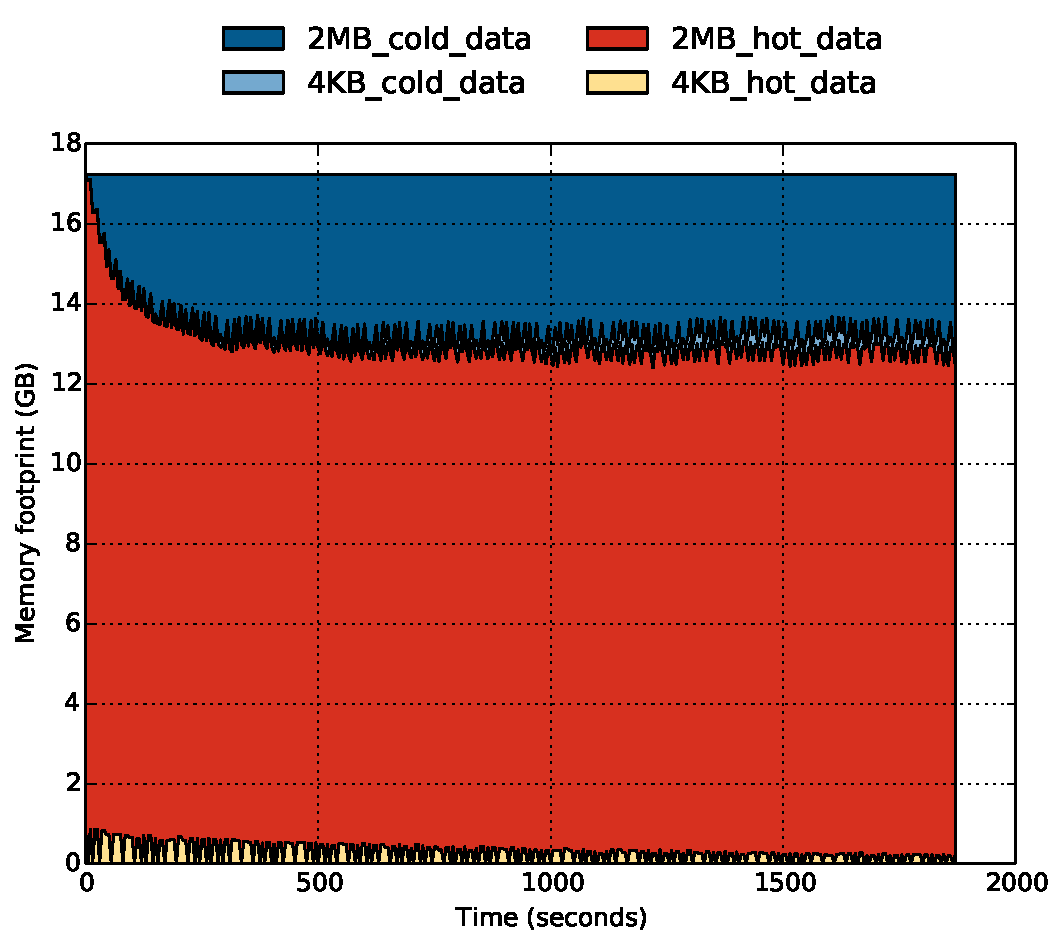
\includegraphics[width=0.8\columnwidth]{asplos2017/figures/redis-skewed-kstaled5-sample5-capacity_over_time.pdf}
\caption{Amount of cold data in Redis identified at run time with 2\%
throughput degradation.}
\label{fig:redis-skewed-hotspot-capacity}
\end{figure}

%\begin{figure}[t]
%\centering
%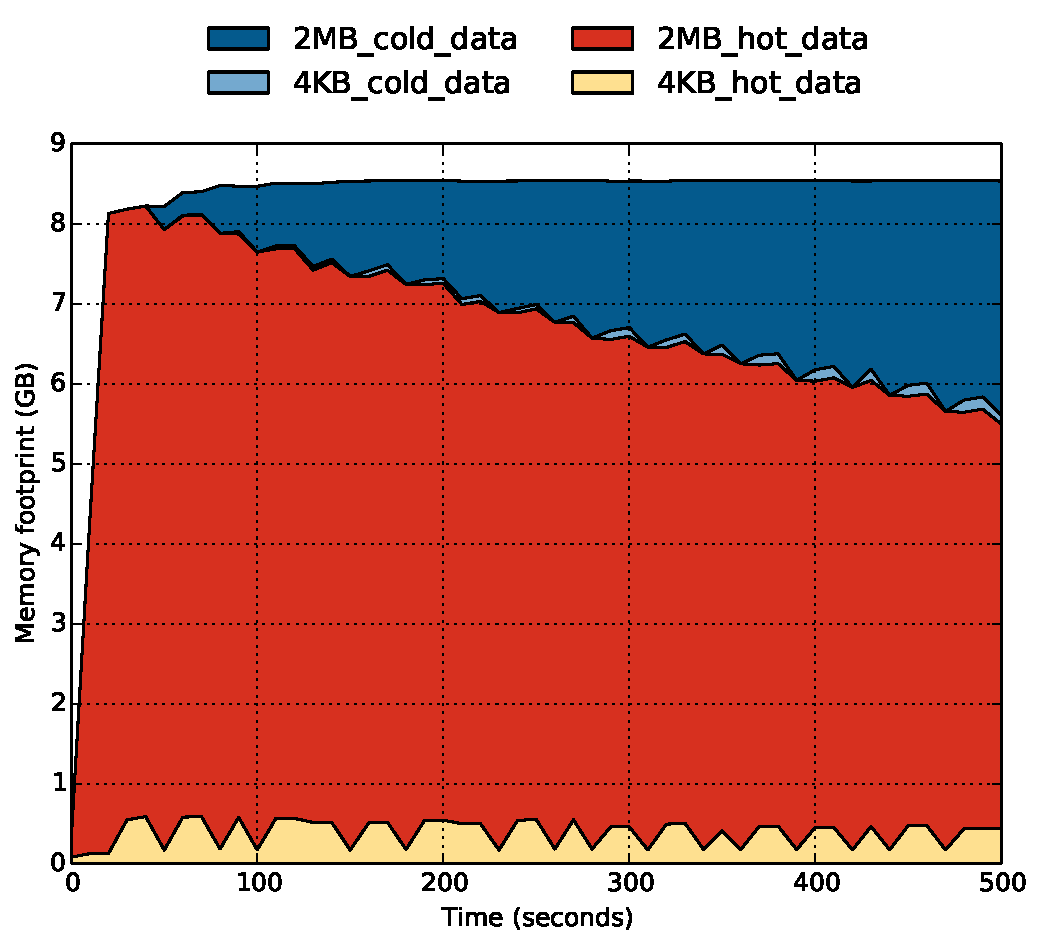
\includegraphics[width=1.0\columnwidth]{figures/ga-new-policy-36cpus-5iter-capacity_over_time.pdf}
%\caption{Amount of cold data in graph analytics benchmark identified at run time with 4\%
%runtime overhead.}
%\label{fig:graph-analytics-capacity}
%\end{figure}
%
\begin{figure}[t]
\centering
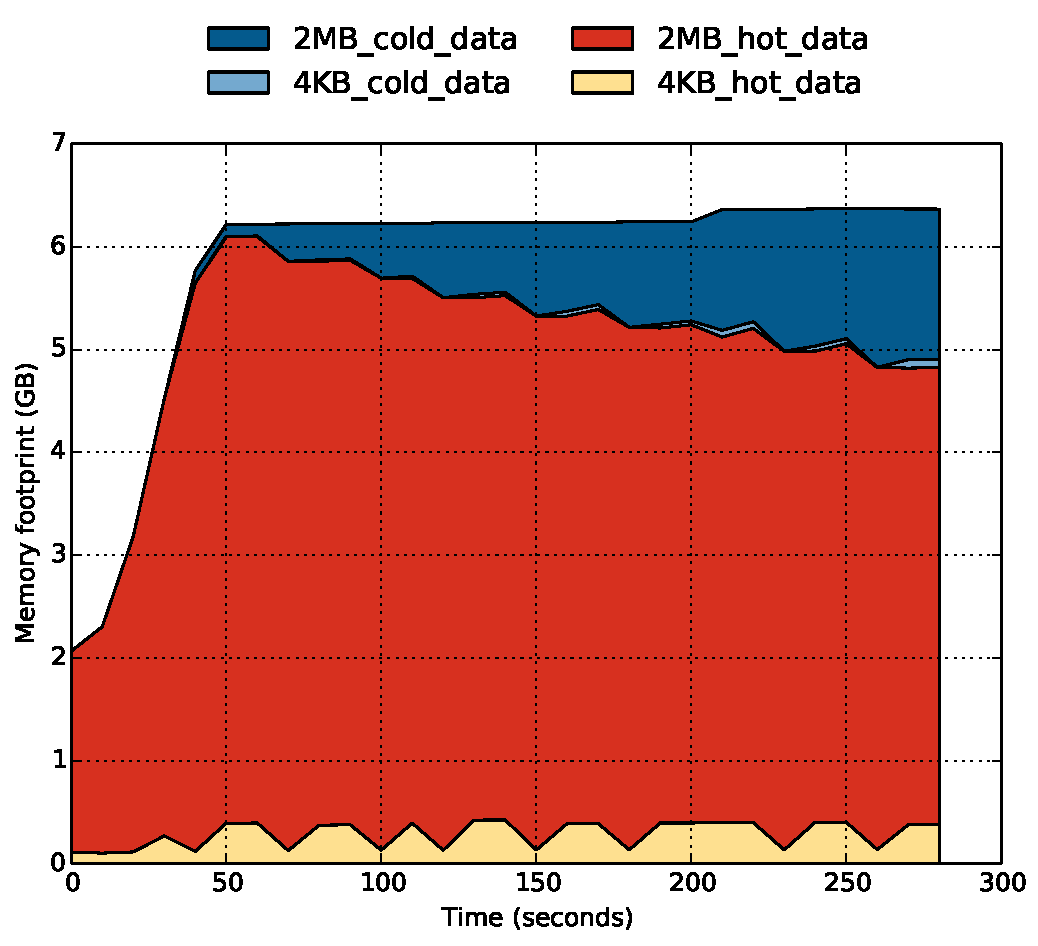
\includegraphics[width=0.8\columnwidth]{asplos2017/figures/ina-6g-new-policy-capacity_over_time.pdf}
\caption{Amount of cold data in in-memory analytics benchmark identified at run
time with 3\% runtime overhead.}
\label{fig:in-memory-analytics-capacity}
\end{figure}

\begin{figure}[t]
\centering
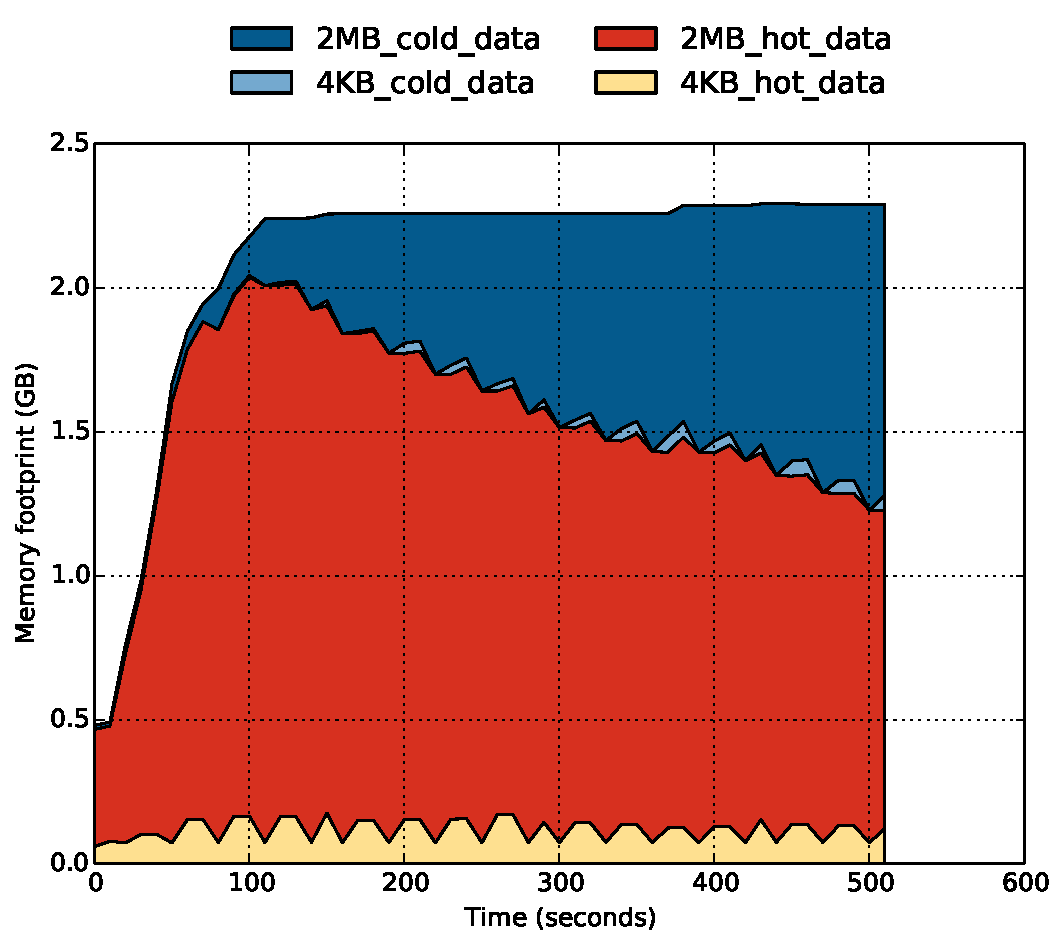
\includegraphics[width=0.8\columnwidth]{asplos2017/figures/wb-hugetmpfs-capacity_over_time.pdf}
\caption{Amount of cold data in web-search benchmark identified at run
time with 1\% throughput and no 99th percentile latency degradation.}
\label{fig:web-search-capacity}
\end{figure}

%\begin{figure}[t]
%\centering
%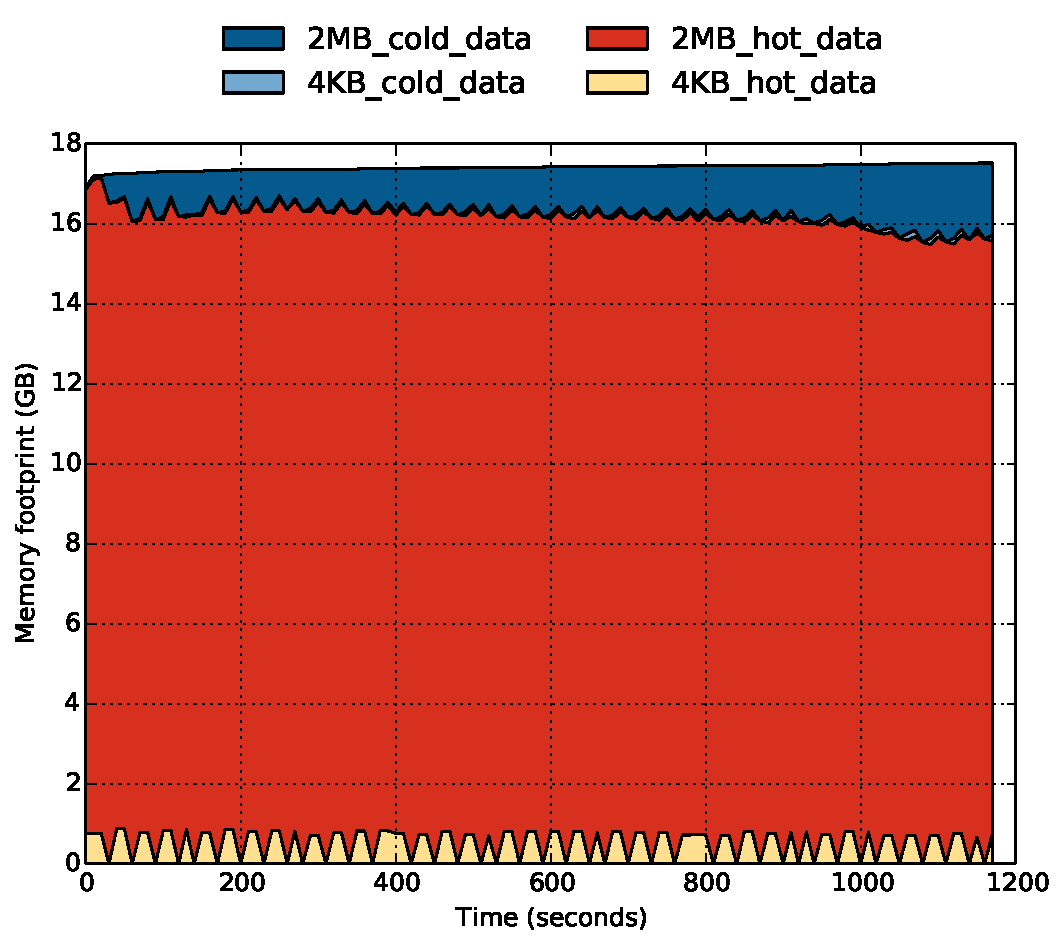
\includegraphics[width=1.0\columnwidth]{figures/redis-new-policy-normal-capacity_over_time.pdf}
%\caption{\fixme{Amount of cold data in Redis identified at run time with 3\%
%throughput degradation.}}
%\label{fig:redis-normal-hotspot-capacity}
%\end{figure}

\begin{figure}[t]
\centering
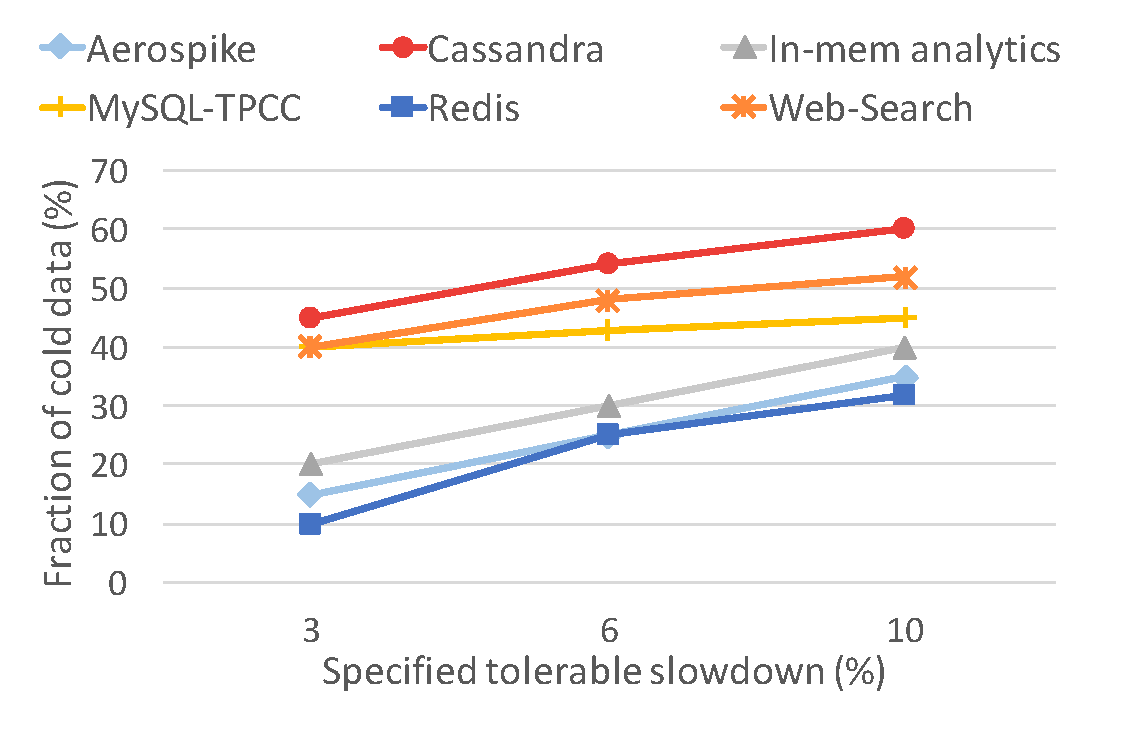
\includegraphics[width=0.8\columnwidth]{asplos2017/figures/slowdown-capacity-sweep.pdf}
\caption{Amount of cold data in identified at run
time varying with the specified tolerable slowdown. All the benchmarks meet
their performance targets (not shown in the figure) while placing cold data in
the slow memory.}
\label{fig:slowdown-capacity}
\end{figure}

%\subsection{Cassandra}
%\label{sec:cassandra}
\textbf{Cassandra}:
We report the breakdown of hot and cold 2MB and 4KB pages over time for 
Cassandra in Figure~\ref{fig:cassandra-capacity} for the write-heavy workload. 
Thermostat identifies between 40-50\% of Cassandra's footprint
(including both 4KB and 2MB pages) as cold. Note that the cold 4KB pages are
solely due to splitting of cold huge pages during profiling ($\approx$ 5\% of
cold pages are 4KB, since our profiling strategy is agnostic of a page being hot
or cold).
Note that the resulting throughput degradation of 2\% falls slightly under our 
target of 3\%. We observe $\approx$ 1\% higher average, 95th, and 99th percentile read/write
latency for Cassandra with Thermostat.
Based on this performance vs. footprint trade-off, we estimate Thermostat 
enables a net cost savings of $\approx$ 30\% for Cassandra (see
Section~\ref{dram-cost} for a detailed analysis). For the read-heavy workload
Thermostat identifies 40\% of data as cold with 2.5\% throughput degradation (we
omit figure due to space constraints).

The memory consumption of Cassandra grows due to in-memory Memtables filling up.
The Memtable is flushed to disk in the form of an SSTable, which then leads to a
sharp decrease in memory consumption. However, we do not observe such a
compaction event in our configuration, due to the large amount of memory
provisioned for Cassandra in our test scenario.

%A distinctive feature of Cassandra's memory footprint is the periodic sawtooth pattern
%visible in the Figure.
%This pattern continues indefinitely if we allow Cassandra to continue to run.
%Cassandra's footprint grows for a period of several hundred seconds as additional entries are 
%appended to its in-memory SSTable cache.  When SSTables grow to a pre-determined
%size, Cassandra invokes a compaction step that consolidates several SSTables into a 
%single file on disk and discards the stale files, leading to a sudden and sharp drop in its
%total footprint in the page cache. Note that the data in these SSTables is extremely cold.
%Hence, Cassandra benefits greatly from shifting a bulk of the page cache to huge pages
%in slow memory.

%\subsection{MySQL-TPCC}
%\label{sec:tpcc}
\textbf{MySQL-TPCC}:
In Figure~\ref{fig:tpcc-capacity} we show a similar footprint graph for MySQL-TPCC. 
The largest table
in the TPCC schema, the LINEITEM table, is infrequently read.  As a result, much
of TPCCs footprint (about 40-50\%) is cold and can be placed in slow memory while
limiting performance degradation to 1.3\%.

%\subsection{Aerospike}
\textbf{Aerospike}:
In Figure~\ref{fig:aerospike-capacity} we show a similar footprint graph for
Aerospike for the read-heavy workload. We see a small fraction of the footprint (about 15\%) identified
as cold while maintaining the tolerable slowdown. The average, 95th and 99th
read/write latencies are all within 3\% of the baseline. For the write-heavy
workload, Thermostat identifies about 15\% of data as cold while satisfying
tolerable slowdown (we omit figure due to space constraints).

%\subsection{Redis}
%\label{sec:redis}
\textbf{Redis}:
Unlike the other applications, Redis has a more uniform access pattern.
The key data structure in Redis is a large hash table, hence, memory accesses
are spread relatively uniformly over its address space; the relative hotness
of pages reflects the corresponding hotness of the key distribution.
We study a load where 0.01\% of keys account for 90\% of accesses.
In Figure~\ref{fig:redis-skewed-hotspot-capacity} we show that, under this load, 10\% of the data is detected as cold at a 3\% throughput degradation. 
The average read/write latency is 3.5\% higher than the baseline.
%There is small fraction of data idenitfied as cold for 3\% tolerable slowdown.
%The input key distribution is skewed, however, due to hashing hot keys are
%uniformly distributed across applicaiton pages. Hence, most pages are detected
%as hot, resulting in very low amount of cold data detection (about 10\%) for
%tolerable 3\% slowdown.

%However, in Figure~\ref{fig:redis-skewed-hotspot-capacity} we show that with a
%highly skewed access pattern as discussed in Section~\ref{sec:benchmarks},
%Thermostat can identify about 25\% as cold while being under tolerable 3\%
%slowdown.Thus, Thermostat successfully identifies cold pages if present in the
%application.

%\subsection{In-memory analytics}
\textbf{In-memory analytics}:
We also evaluate in-memory analytics benchmark from
Cloudsuite~\cite{cloudsuite}.  In Figure~\ref{fig:in-memory-analytics-capacity}
we show Thermostat detects about 15-20\% data as cold. As application footprint
grows, Thermostat scans more pages and thus the cold page fraction also grows with time.
We run this benchmark to completion, however, the benchmark runtime is much shorter
than the previous data serving applications. (Cloudsuite is 
designed for tractable runtimes under expensive instrumentation and/or simulation). 
Nevertheless,  Thermostat successfully identifies cold data while meeting the
slowdown target.  We expect the cold memory footprint of this application to 
reach steady state if a larger input were available.

%\subsection{Web search}
\textbf{Web search}:
In Figure~\ref{fig:web-search-capacity} we show the footprint graph for the web search workload. We see about 40\% of the footprint identified as cold. 
We observe $<$ 1\% degradation in throughput and no observable degradation in 99th
percentile latency of 200ms.

%\subsection{Sensitivity to hot-cold classification}
%To form a more complete picture of the trade-off between the fraction of memory
%classified as cold and performance degradation, we sweep a range of Thermostat
%classification thresholds and report the resulting trade-offs in Figure~\ref{fig:throughput-capacity}.
%The horizontal access reports the fraction of memory classified as cold while the
%vertical axis reports the corresponding throughput degradation for each of the three
%applications.
%
%TPCC is relatively insensitive to main memory access latency.  It incurs less than 
%5\% throughput degradation even when mapping 90\% of data to slow memory.
%%\fixme{Doesn't this result sort of imply your classification sucks?  Shouldn't you be classifying more stuff as cold?  This result seems awfully fishy.}
%In contrast, Redis is extremely sensitive to main memory access latency, slowing
%by more than 10\% if more than 40\% of its memory footprint is classified as cold.
%Cassandra is relatively tolerant of slower memory access except for about 20\%
%of its footprint, which is extremely hot and incurs drastic slowdown if shifted
%to slow memory.
%
%Figure~\ref{fig:cdf-sample2} also shows that Redis has two categories of
%pages (corresponding to two steep slopes in the CDF): one colder category with
%$\approx$ 100-200 hot 4KB pages, and another hotter category with $\approx$
%300-400 hot 4KB pages. Na\"{\i}vely, one would assume that the entirety of the
%``cold''-er data can be placed in slow memory. However, an accurate evaluation with our
%evaluation methodology shows that only about 40\% of that memory can actually be
%mapped to slow memory without suffering significant throughput degradations --
%highlighting the utility of an application-transparent and
%hardware-investment-free approach.
%

%\subsection{Sensitivity to tolerable slowdown}
%
%\subsection{Sensitivity to slow memory latency}
%\begin{figure}[t]
%\centering
%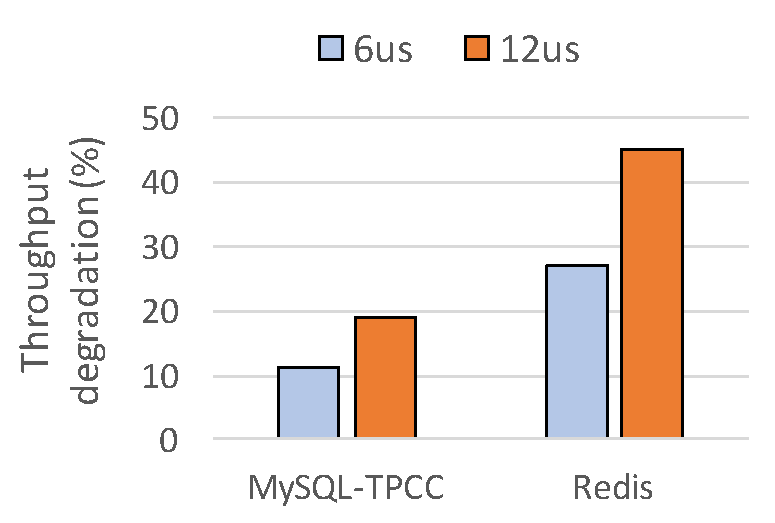
\includegraphics[width=1.0\columnwidth]{figures/latency-sweep.pdf}
%\caption{Slow memory latency sweep for 6 $\mu$s and 12 $\mu$s. Cassandra's throughput
%drops to 0 multiple times in between the run because of such high latencies.
%(Lower is better).}
%\label{fig:latency-sweep}
%\end{figure}
%
%As the access latency of future memory technologies remains uncertain, we perform
%a sensitivity study where we substantially increase the slow-memory access latency to
%6 and 12 microseconds.  We select these values to represent prior work on 
%disaggregated memory~\cite{Lim2012} where slow-memory accesses must 
%traverse a high-latency interconnect. Figure~\ref{fig:latency-sweep} shows the resulting 
%throughput degradation for Redis and TPCC. Cassandra fails to complete under these
%settings, due to application timeouts, so we omit its results. We can see that whereas TPCC can
%withstand a memory latency of 6 $\mu$s with $<$ 10\% throughput
%degradation, none of the applications can withstand 12 $\mu$s slow memory
%latency without significant throughput degradation. This observation points to
%the unsuitability of cache-line-grained accesses for such high memory latencies.


\subsection{Sensitivity to tolerable slowdown target}
Next we show the sensitivity of Thermostat to the single input parameter
specified by a system administrator, the tolerable slowdown. In our baseline evaluation, we set this parameter to 3\%. However, due to changes in the
price point of the memory technology or changes in data-center cost structure
it may be  possible to tolerate higher slowdown. To study the adaptability of
Thermostat in such scenarios we also evaluate 6\% and 10\% slowdown targets. We show the variation in amount of cold data identified by
Thermostat at run time with tolerable slowdown in Figure~\ref{fig:slowdown-capacity}.

We observe that with increase in tolerable slowdown Thermostat can place a higher
fraction of memory footprint in slow memory. We also observe
that the performance targets of all applications are met (we omit data due to space
constraints). However, in several cases, the achieved slowdown is less than the
specified slowdown.
%For Redis, Thermostat is able to identify higher
%fraction of cold data for higher tolerable slowdown as well as observed slowdown
%tracks the specified tolerable slowdown.

For MySQL-TPCC, Thermostat is not able to identify additional cold data even with
an increase in tolerable slowdown (cold data fraction saturates at $approx$ 45\%).
This saturation happens because all remaining pages for TPCC are highly accessed, and
placing any of them in slow memory results in an unacceptable application
slowdown.
%due to a sharp increase in memory access rate of pages in the application, which
%if migrated to slow memory will result in slowdown beyond tolerable, violating
%performance guarantees.
For Aerospike, Thermostat is able to scale the cold data
with varying tolerable slowdown. However, the actual slowdown doesn't reach the
target slowdown due to (a) Aerospike's performance being insensitive to cold page
accesses, and (b) the average OS fault handler latency for emulation being lower
than the assumed latency of 1us used in Thermostat.
%We attribute this observation to the fact that slow memory latency
%emulated in our platform depends on the page fault handler latency whose latency
%is not exactly 1us (lower in case of Aerospike), forcing Thermostat to
%pessimestically place smaller fraction of application data in slow memory. Note
%that on a platform with physical slow memory this problem will not be exhibited.

In summary, Thermostat places a higher fraction of data in slow memory if
the user can tolerate more slowdown. This feature
allows system administrators to better utilize expensive DRAM capacity by moving
as much cold data to slow memory as possible via Thermostat.

\subsection{Migration overhead and slow memory access rate}
\begin{table}
\begin{center}
\begin{tabular}{|c|c|c|}
%\begin{tabular}{|p{0.25\columnwidth}|c|c|}
\hline
(MB/s)&Migration& False-classification\\
\hline
Aerospike & 13.3& 9.2\\
\hline
Cassandra & 9.6 & 3.8\\
\hline
%Graph-Analytics & 7.5& 0.9\\
%\hline
In-mem-Analytics & 16& 0.4\\
\hline
MySQL-TPCC & 6 & 1.8\\
\hline
Redis & 11.3& 10\\
\hline
Web-search & 1.6 & 0.3\\
\hline
\end{tabular}
\caption{Data migration rate and false classification rate of slow memory. These rates are
well-below expected bandwidth of near-future memory technologies.}
\label{tab:nvm-access-rate}
\end{center}
\vspace{-0.15in}
\end{table}

To verify that Thermostat doesn't cause un-realizable bandwidth pressure on the
slow memory, we measured the memory bandwidth required by migrations and false
classifications between slow and fast memory.  In
Table~\ref{tab:nvm-access-rate} we observe that the required migration bandwidth
is $<$ 30 MB/s on average across all benchmarks.  The highest total traffic to
cold memory we observe is 60 MB/s, which is well within the projected capability
of near-future cheap memory technologies~\cite{ref:Dulloor:datatiering}. Thus,
we infer that Thermostat doesn't produce unrealistic pressure on the memory
system.

\subsection{DRAM Cost Analysis}
\label{dram-cost}
Since DRAM pricing is volatile, and slow memory prices remain unclear, it is difficult
to perform a rigorous cost-savings analysis for Thermostat.  We use a simple
model to estimate the cost-savings possible with Thermostat and study a range of 
possible ratios of DRAM to slow-memory cost.
Table~\ref{tab:cost-analysis} shows the fraction of DRAM spending
saved due to Thermostat when slow memory is $\frac{1}{3}$, $\frac{1}{4}$ and
$\frac{1}{5}$ of DRAM cost. We can see that, depending on workload and memory
technology, anywhere from $\approx$ 10\% (for Aerospike) to 32\% (for Cassandra)
of DRAM cost can be saved.

\begin{table}
\begin{center}
\begin{tabular}{|p{0.35\columnwidth}|c|c|c|}
\hline
Slow memory cost relative to DRAM&$0.33\times$& $0.25\times$ & $0.2\times$\\
\hline
Aerospike & 10\% & 11\% & 12\% \\
\hline
Cassandra & 27\% & 30\% & 32\% \\
\hline
In-mem-Analytics & 11\% & 12\% & 13\% \\
\hline
MySQL-TPCC & 27\% & 30\% & 32\% \\
\hline
Redis & 17\% & 19\% & 20\% \\
\hline
Web-search & 27\% & 30\% & 32\% \\
\hline
\end{tabular}
\caption{Memory spending savings relative to an all-DRAM system when using slow
memory with different cost points relative to DRAM.}
\label{tab:cost-analysis}
\end{center}
\vspace{-0.15in}
\end{table}


\subsection{Related Work}
\label{related_work}
%\vspace{-0.05in}
With the introduction of symmetric multiprocessors, significant work has examined optimal placement of processes and memory
in CC-NUMA systems~\cite{Wilson2001,Bolosky1989,Brecht1993,LaRowe1992,Verghese1996,Iyer1998}.
While much of this early work focused on placing processes and data in
close proximity to each other,  more recent work has recognized that
sharing patterns, interconnect congestion, and even queuing
delay within the memory controller are important metrics to consider when
designing page and process placement policies~\cite{AUTONUMA,Dashti2013,Tam2007,Zhuravlev2010,Knauerhase2008,Blagodurov2011,awasthinellans10}.
Nearly all of these works focus on improving traditional CPU throughput
where reduced memory latency is the primary driver of memory system performance.
Recent work from Gerofi et al.~\cite{Gerofi2014} examines TLB replacement policies for the Xeon Phi
co-processor with a focus on highly parallel applications with large data
footprints.

Using non-DRAM technologies or mixed DRAM technologies for main memory systems to improve power
consumption on traditional CPUs has also been
explored by several groups~\cite{Kultursay2013,Phadke11mlpaware2011,Mogul2009,Bheda2011,Ramos2011,Nil2012,pavlovic2013}.  
Much of this work has focused on overcoming the performance
peculiarities that future non-volatile memory (NVM) technologies may have compared to existing DRAM designs.
In addition to mixed technology off-package memories, upcoming on-package memories provide opportunities
for latency reduction by increasing the number of banks available to the application~\cite{Dong2010}
and may one day be configurable to balance bandwidth application needs with power
consumption~\cite{Zhao2012}.
An alternative to treating heterogeneous memory systems as a flat
memory space is to use one technology as a cache for the other~\cite{jiang2011,Meza2012}.  While this
approach has the advantage of being transparent to the programmer, 
{\color{black}OS, and runtime systems}, 
few implementations~\cite{Sim2012} take advantage of the additive bandwidth available
when using heterogeneous memory.

In the GPU space, Zhao et al.~\cite{zhao2013} have explored the affect 
of hybrid DRAM-NVM systems on GPU compute workloads, making the observation that modern GPU designs are very
good at hiding variable memory system latency. Wang et al.~\cite{Wang2013} explore a mixed NVM-DRAM
system that uses compiler analysis to identify near-optimal data placement across kernel invocations
for their heterogeneous memory system. While their system 
does not significantly improve performance, it offers improved power 
efficiency through use of NVM memory and shows that software based page 
placement, rather than hardware caching, can be a viable 
alternative to managing heterogeneous memory for use with GPUs.

\section{Conclusion}
\label{conclusion}


%%%%%%% -- PAPER CONTENT ENDS -- %%%%%%%%

%%%%%%%%% -- BIB STYLE AND FILE -- %%%%%%%%
\bibliographystyle{ieeetr}
\bibliography{ref}
%%%%%%%%%%%%%%%%%%%%%%%%%%%%%%%%%%%%

\end{document}
